\documentclass[11pt,a4paper]{article}

\usepackage[T1]{fontenc}
\usepackage[utf8]{inputenc}
\usepackage[margin=2.2cm]{geometry}
\usepackage{amsmath,amssymb}
\usepackage{booktabs}
\usepackage{array}
\usepackage{enumitem}
\usepackage{tikz}
\usepackage[hidelinks]{hyperref}

\setlist{itemsep=1pt,topsep=3pt,parsep=0pt}
\setcounter{tocdepth}{2}
\setcounter{secnumdepth}{3}

\title{CSE 753 --- Advanced Reinforcement Learning\\[4pt]
\large Comprehensive Final Examination Study Notes\\[2pt]
\normalsize Lectures 06--09: Policy Gradients, Actor--Critic, Imitation Learning
and Offline RL, Reward Learning and RLHF}
\author{Prepared as course study material}
\date{}

\begin{document}
\maketitle
\sloppy

\tableofcontents
\newpage

%=====================================================================
\section{Part I --- Policy Gradient Methods (Lecture 06)}
%=====================================================================

\subsection{The setting: why learn a policy directly at all?}

\paragraph{What it is.} Everything before this lecture was
\emph{generalised policy iteration}: maintain $Q(s,a)$, and derive the policy
from it by acting greedily. Policy gradient methods throw the intermediate
step away. You parameterise the policy itself as
$\pi(a\mid s,\theta)=\Pr\{A_t=a\mid S_t=s,\theta_t=\theta\}$, with
$\theta\in\mathbb R^{d'}$, and improve $\theta$ by gradient ascent on
performance.

\paragraph{Plain English.} Instead of learning ``how good is each action here''
and then picking the best, you learn ``what should I do here'' directly, and
nudge that behaviour up or down according to how well things turned out.

\paragraph{What problem it solves.} Three things. (i) In continuous or very
large action spaces, $\arg\max_a Q(s,a)$ is itself a hard optimisation
problem at every step; a parameterised policy just outputs the action.
(ii) The policy is often a simpler object than the value function --- knowing
\emph{that} you should brake is easier than knowing the exact discounted
return of braking. (iii) It gives you \emph{stochastic} policies natively,
which value-greedy methods cannot represent.

\paragraph{What it cannot solve.} It gives no value estimate, so it has no
mechanism for credit assignment beyond ``the whole trajectory turned out
well''. That gap is precisely what Lecture~07 fills.

\paragraph{What problems it gave rise to.} High variance, on-policy-only data,
and sample inefficiency --- the three themes of the rest of the lecture.

\subsection{Policy parameterisation and the softmax policy}

\paragraph{What it is.} Any parameterisation must satisfy
$\pi(a\mid s,\theta)\ge 0$ for all $a,s$ and $\sum_{a\in\mathcal A}\pi(a\mid s,\theta)=1$
for all $s$. For discrete actions the standard construction is the softmax
over \emph{action preferences} $h(s,a,\theta)$:
\[
\pi(a\mid s,\theta)=\frac{e^{h(s,a,\theta)}}{\sum_{b\in\mathcal A}e^{h(s,b,\theta)}}.
\]

\paragraph{Plain English.} The network outputs one unnormalised score per
action; the exponential makes those scores positive and the denominator makes
them sum to one. The scores are called preferences because their
\emph{absolute} value is meaningless --- only differences between them matter.

\paragraph{The key behavioural fact.} As the preference $h(s,a,\theta)$ of one
action grows large relative to the others, the softmax tends towards
\emph{greedy}: it puts almost all probability on that action. This is the
link between parameter magnitude and exploration. A policy that has been
trained for a long time has large preferences and therefore explores little,
without anyone having explicitly scheduled an exploration parameter.

\paragraph{Advantages.} Smooth in $\theta$, so gradients exist everywhere;
naturally normalised; can approach determinism arbitrarily closely without
ever becoming discontinuous.

\paragraph{Disadvantages.} It can \emph{only} approach determinism
asymptotically, so it can be slow to commit; and because only differences of
preferences matter, the parameterisation is over-specified (adding a constant
to every $h$ changes nothing), which can make optimisation ill-conditioned.

\paragraph{What if it had been done differently?} If you parameterised the
probabilities directly and projected onto the simplex, you would have to
handle the constraint explicitly at every step and you would lose
differentiability at the simplex boundary. The exponential is there to turn a
constrained problem into an unconstrained one.

\paragraph{Exam hook.} ``As the action preference $h(s,a,\theta)$ grows, how
does the policy behave?'' Answer: it tends towards greedy action selection,
which also means exploration decays as parameters grow.

\subsection{Why stochastic policies: the state-aggregation argument}

\paragraph{What it is.} A claimed advantage of policy parameterisation is that
it can represent stochastic policies, and under function approximation the
best stochastic policy can be \emph{strictly better} than the best
deterministic one.

\paragraph{The lecture's example.} A short corridor of three states leading to
a goal $G$, reward $-1$ per step, where in the middle state the effects of the
two actions are \emph{reversed}. Crucially, all three states are
\emph{aggregated} --- the function approximator cannot tell them apart, so it
must emit the same action distribution in all three.

\paragraph{Plain English.} If you cannot distinguish two states, and the right
action differs between them, then \emph{any} deterministic rule is wrong in at
least one of them, and being wrong there can trap you (you loop forever). A
coin-flipping policy is wrong sometimes in both, but never traps you. Mixing
is strictly better than committing when you are blind.

\paragraph{The number to quote.} The best stochastic policy under aggregation
puts roughly $59\%$ of its mass on ``right'' and $41\%$ on ``left'', achieving
$V_{\pi_\theta}(s)=-11.6$. Both deterministic policies do far worse. (I
verified this by solving the linear system for the aggregated chain: the
optimum sits at $p\approx0.59$ with $V\approx-11.66$.)

\paragraph{What problem it solves.} Partial observability and function
approximation error. Randomisation is a hedge against not knowing which state
you are in.

\paragraph{What it cannot solve.} It does not recover the information you lost.
The stochastic optimum is still much worse than the true optimum with full
state information. Randomising is damage limitation, not a fix.

\paragraph{When to use it.} Whenever the representation cannot distinguish
states that require different actions --- partial observability, aggressive
state aggregation, adversarial settings where predictability is exploitable.

\paragraph{When not to.} In a fully observed, tabular MDP the optimal policy is
deterministic; stochasticity there is pure loss.

\paragraph{Exam hook.} A one-line justification part. Say: ``under function
approximation with state aggregation, the best deterministic policy can be
strictly worse than the best stochastic one --- the corridor example gives
$V_{\pi_\theta}=-11.6$ for the $41\%/59\%$ mixture.''

\subsection{The RL objective and its gradient}

\paragraph{The objective.}
\[
\theta^\star=\arg\max_\theta \mathbb E_{\tau\sim p_\theta(\tau)}[r(\tau)],
\qquad
J(\theta)=\mathbb E_{\tau\sim p_\theta(\tau)}\!\left[\sum_t r(s_t,a_t)\right]
\approx \frac1N\sum_i\sum_t r(s_{i,t},a_{i,t}),
\]
where the approximation is a Monte Carlo average over $N$ trajectories sampled
\emph{from} $\pi_\theta$. That last clause is the whole on-policy story in
miniature.

\paragraph{The derivation --- reproduce this chain.}
\begin{align}
J(\theta) &= \int p_\theta(\tau)\,r(\tau)\,d\tau \\
\nabla_\theta J(\theta) &= \int \nabla_\theta p_\theta(\tau)\,r(\tau)\,d\tau
&&\text{(reward does not depend on $\theta$)}\\
&= \int p_\theta(\tau)\,\nabla_\theta \log p_\theta(\tau)\,r(\tau)\,d\tau
&&\text{(log-derivative trick)}\\
&= \mathbb E_{\tau\sim p_\theta}\!\left[\nabla_\theta\log p_\theta(\tau)\,r(\tau)\right].
\end{align}
The log-derivative trick is the identity
$p_\theta(\tau)\nabla_\theta\log p_\theta(\tau)
= p_\theta(\tau)\frac{\nabla_\theta p_\theta(\tau)}{p_\theta(\tau)}
= \nabla_\theta p_\theta(\tau)$.
Its purpose is to turn $\int \nabla_\theta p_\theta(\tau)(\cdot)d\tau$, which
is not an expectation and cannot be sampled, back into an expectation under
$p_\theta$, which \emph{can} be sampled.

\paragraph{Why the dynamics vanish --- say this in one sentence.} Expand
\[
\log p_\theta(\tau)=\log p(s_1)+\sum_{t=1}^T \log\pi_\theta(a_t\mid s_t)
+\sum_{t=1}^T \log p(s_{t+1}\mid s_t,a_t).
\]
The initial-state term and the transition terms do not depend on $\theta$, so
they die under $\nabla_\theta$. \textbf{This is why policy gradient is
model-free}: you never need to know or estimate $p(s_{t+1}\mid s_t,a_t)$.

\paragraph{The final estimator.}
\[
\nabla_\theta J(\theta)\approx
\frac1N\sum_{i=1}^N\left(\sum_{t=1}^T \nabla_\theta\log\pi_\theta(a^i_t\mid s^i_t)\right)
\left(\sum_{t=1}^T r(s^i_t,a^i_t)\right).
\]

\paragraph{How to read the estimator (this single sentence answers most of Section 1).}
It is a \textbf{weighted maximum-likelihood update, not a descent on a loss}.
The vector $\nabla_\theta\log\pi_\theta(a\mid s)$ is the direction in
parameter space that makes the action you actually took \emph{more likely};
the return is a scalar deciding how far to move in that direction and with
what sign. Positive return $\Rightarrow$ do more of that. Negative return
$\Rightarrow$ do less.

\paragraph{Properties.} The estimator is \textbf{unbiased} but
\textbf{high-variance}. Every later technique in this course trades a little
bias for a large reduction in variance, or spends computation to reduce
variance without adding bias.

\subsection{REINFORCE (vanilla policy gradient)}

\paragraph{The algorithm.}
\begin{enumerate}[label=\arabic*.]
\item Sample $\{\tau^i\}$ from $\pi_\theta(a_t\mid s_t)$.
\item $\nabla_\theta J(\theta)\approx \sum_i\left(\sum_{t=1}^T\nabla_\theta\log\pi_\theta(a^i_t\mid s^i_t)\right)\left(\sum_{t=1}^T r(s^i_t,a^i_t)\right)$.
\item $\theta \leftarrow \theta+\alpha\nabla_\theta J(\theta)$.
\item Repeat until convergence.
\end{enumerate}

\paragraph{What problem it solves.} It gives an unbiased, model-free way to
improve a policy in an arbitrary MDP, including continuous actions, with no
value function and no knowledge of dynamics.

\paragraph{What it cannot solve.}
\begin{itemize}
\item \textbf{Credit assignment within a trajectory.} Every action in a
trajectory gets the \emph{same} scalar weight --- the total return. A good
action in a bad trajectory is punished; a bad action in a good trajectory is
reinforced.
\item \textbf{Variance.} The weight is a sum of many random rewards, so its
spread is enormous, and the gradient estimate is dominated by noise.
\item \textbf{Reward-scale sensitivity.} Add $+1000$ to every reward and the
optimal policy is unchanged, but every weight becomes hugely positive and the
algorithm reinforces everything, including failures.
\item \textbf{Sample reuse.} It is on-policy; a single batch buys a single
gradient step.
\end{itemize}

\paragraph{Exam hook --- the three quiz slides, which are three distinct failures.}

\begin{center}
\begin{tabular}{@{}p{0.30\linewidth}p{0.32\linewidth}p{0.30\linewidth}@{}}
\toprule
\textbf{Symptom} & \textbf{Cause} & \textbf{Fix on the slides} \\
\midrule
Whole trajectory uniformly reinforced or punished; a step forward gets pushed
down because the robot later fell backwards &
No credit assignment across $t$; every action weighted by the total return &
Reward-to-go \\
\addlinespace
All four trajectories succeed, so all weights are positive and behaviour that
is merely less bad is still reinforced &
Returns are all positive; the estimator is noisy and sensitive to reward scale &
Baseline \\
\addlinespace
Jacket folding with $r\in\{0,0.5,1\}$: gradient weight is essentially constant
across trajectories &
Sparse reward --- almost every trajectory receives $0$ &
Baseline helps, but the real fix is a learned critic (Lecture 07) \\
\bottomrule
\end{tabular}
\end{center}

\noindent\textbf{Note on the second row.} The lecture slide for the
all-successes case reuses the answer text of the first slide. Do not copy that
first sentence; the actual point of that slide is the \emph{second} sentence:
policy gradient is noisy, high-variance and sensitive to reward scale.

\subsection{Reward-to-go}

\paragraph{What it is.} Replace the trajectory return in the weight by the sum
of rewards \emph{from the current timestep onwards}:
\[
\nabla_\theta J(\theta)\approx \frac1N\sum_i\sum_{t=1}^T
\nabla_\theta\log\pi_\theta(a^i_t\mid s^i_t)
\left(\sum_{t'=t}^{T} r(s^i_{t'},a^i_{t'})\right),
\qquad
\hat Q^i_t \;=\; \sum_{t'=t}^{T} r(s^i_{t'},a^i_{t'}).
\]
Note the limit: the sum starts at $t'=t$, \textbf{inclusive}.

\paragraph{Plain English.} Judge an action by what happened after it, not by
what happened before it. Anything that occurred earlier in the trajectory is
not that action's fault or credit.

\paragraph{The justification, in one line.} \emph{Policy behaviour at time $t$
cannot affect rewards at times $t'<t$} --- causality. Dropping those terms
therefore removes noise without introducing bias.

\paragraph{What problem it solves.} Partial credit assignment across time, and
a genuine variance reduction (fewer random terms in each weight).

\paragraph{What it cannot solve.} It still cannot separate a \emph{bad action}
from a \emph{good outcome that happened to follow it}. If an action moves you
away from the goal but a large reward arrives two steps later, reward-to-go
credits the bad action with that reward. This is exactly the trap in
Scenario~1 Q3 of the practice paper.

\paragraph{What problem it gave rise to.} Nothing new --- it is a strict
improvement. But by making the weights \emph{differ} across timesteps it
exposes the next issue: the weights are still all positive when all rewards
are positive.

\paragraph{Counterfactual.} If you summed from $t+1$ instead of $t$, you would
be judging the action by everything except its own immediate consequence ---
throwing away the most informative single term. If you summed from $t'=1$ you
would be back to REINFORCE. The inclusive lower limit is load-bearing; the
examiner checks it.

\paragraph{Worked pattern (practice paper).} Rewards
$\tau_1=(+1,+10)$, $\tau_2=(-1,+10)$, $\tau_3=(+1,-1)$, $\tau_4=(-1,-1)$.
\[
\hat Q^1=(11,10),\quad \hat Q^2=(9,10),\quad \hat Q^3=(0,-1),\quad \hat Q^4=(-2,-1).
\]
Practise building this table quickly: the $t=2$ entry is just $r_2$; the $t=1$
entry is $r_1+r_2$.

\subsection{Baselines}

\paragraph{What it is.} Subtract a constant from the weight:
\[
\nabla_\theta J(\theta)=\mathbb E_{\tau\sim p_\theta}\!\left[
\nabla_\theta\log p_\theta(\tau)\,\bigl(r(\tau)-b\bigr)\right],
\qquad
b=\frac1N\sum_{i=1}^N r(\tau_i).
\]

\paragraph{Plain English.} ``Was this better or worse than average?'' rather
than ``was this good?''. Only above-average behaviour gets reinforced;
below-average behaviour gets actively pushed down, even when its raw return
was positive.

\paragraph{The unbiasedness proof --- memorise the four-step chain.}
\[
\mathbb E\bigl[\nabla_\theta\log p_\theta(\tau)\,b\bigr]
=\int p_\theta(\tau)\nabla_\theta\log p_\theta(\tau)\,b\,d\tau
=\int \nabla_\theta p_\theta(\tau)\,b\,d\tau
= b\,\nabla_\theta\!\int p_\theta(\tau)\,d\tau
= b\,\nabla_\theta 1 = 0 .
\]
The load-bearing step is the last one: the constant survives the expectation
only because the density integrates to one, so its gradient is the gradient of
a constant. \textbf{Subtracting a constant baseline changes the variance but
not the expectation.}

\paragraph{What problem it solves.} (i) Removes the ``everything is positive,
so reinforce everything'' failure. (ii) Reduces variance. (iii) Removes
sensitivity to an additive shift of the reward function.

\paragraph{What it cannot solve.}
\begin{itemize}
\item It \textbf{reduces} variance; it does not remove it. Say ``reduce'', not
``eliminate''.
\item A \emph{constant} baseline is state-independent. It cannot answer ``was
this action better than what my policy usually does \emph{in this state}?'',
which is the question that actually matters for credit assignment. That gap is
what the advantage function $A^\pi(s,a)$ in Lecture~07 exists to close.
\item Under sparse rewards the baselined weight is near-constant across almost
all trajectories, so it barely helps. This motivates a learned critic.
\end{itemize}

\paragraph{Counterfactual.} If $b$ depended on the \emph{action}, the proof
would fail: $b(a)$ could not be pulled outside the integral over $\tau$ and
the estimator would become biased. This is precisely why the baseline may
depend on the state (giving $V^\pi(s)$ and hence the advantage) but never on
the action. That is a strong E4 answer if asked why $V$ and not $Q$ is used as
a baseline.

\paragraph{Sign reading (E2 --- this is most of Section 1).}
\[
\hat Q^i_t - b > 0 \;\Rightarrow\; \text{gradient \emph{increases} } \log\pi_\theta(a^i_t\mid s^i_t);
\qquad
\hat Q^i_t - b < 0 \;\Rightarrow\; \text{it \emph{decreases} it.}
\]

\paragraph{Worked pattern.} Continuing the warehouse table: the eight
reward-to-go samples are $\{11,10,9,10,0,-1,-2,-1\}$, so
$b=\tfrac{36}{8}=4.5$. Then, for example, $\tau_3$ at $t=1$ has
$0-4.5=-4.5<0$ (log-probability \emph{decreased}) and $\tau_4$ at $t=2$ has
$-1-4.5=-5.5<0$ (also decreased).

\subsection{On-policy invalidity --- the boundary you must hold}

\paragraph{What it is.} $J(\theta)$ is an expectation over $\tau\sim p_\theta$.
The Monte Carlo estimate is only valid for the $\theta$ that generated the
samples. The moment you take one gradient step, $\theta$ has moved, and the
stored trajectories are draws from the \emph{wrong} distribution.

\paragraph{Say it precisely.} Reusing a batch is not merely
\emph{inefficient}; the estimator becomes \textbf{biased} --- it is an
estimator of the gradient of the wrong objective. This distinction is what a
question about ``reuse the four trajectories for five more gradient steps''
is testing.

\paragraph{Consequence.} One batch of environment interaction buys exactly one
gradient step. For a real robot or a hospital, this is prohibitively expensive.

\subsection{Importance sampling and the off-policy policy gradient}

\paragraph{What it is.} Reweight each old sample by how much more or less
likely it is under the new policy. At the trajectory level:
\[
\nabla_{\theta'}J(\theta')=\mathbb E_{\tau\sim p_\theta(\tau)}\!\left[
\prod_{t=1}^{T}\frac{\pi_{\theta'}(a_t\mid s_t)}{\pi_\theta(a_t\mid s_t)}
\left(\sum_{t=1}^{T}\nabla_{\theta'}\log\pi_{\theta'}(a_t\mid s_t)\right)
\left(\sum_{t'=t}^{T} r(s_{t'},a_{t'})-b\right)\right].
\]

\paragraph{Plain English.} If the new policy would have chosen this action
twice as often as the old one, count this sample twice. That converts data
from the old policy into a valid (if noisier) estimate for the new one.

\paragraph{The failure --- this is the standard E5 answer.} The trajectory
ratio is a \textbf{product of $T$ terms}. A product of many numbers each
slightly above or below one either explodes or collapses towards zero, and its
\emph{variance grows exponentially in the horizon}. State it as: \emph{for
long trajectories, or for a policy that has moved far from $\pi_\theta$, the
product of $T$ ratios has variance growing exponentially with $T$, so the
estimate becomes useless.}

\paragraph{The per-timestep repair (the final form on the slides).}
\[
\nabla_{\theta'}J(\theta')\approx
\frac1N\sum_{i=1}^N\sum_{t=1}^{T}
\frac{\pi_{\theta'}(a_{i,t}\mid s_{i,t})}{\pi_\theta(a_{i,t}\mid s_{i,t})}
\nabla_{\theta'}\log\pi_{\theta'}(a_{i,t}\mid s_{i,t})
\left(\sum_{t'=t}^{T} r(s_{i,t'},a_{i,t'})-b\right).
\]
The slides pass through an intermediate form with a \emph{state--action
marginal} ratio $\tfrac{\pi_{\theta'}(s_{i,t},a_{i,t})}{\pi_\theta(s_{i,t},a_{i,t})}$,
note that it is ``much less likely to explode or vanish, but hard to
measure'' --- you cannot compute a state marginal --- and then drop the state
part to reach the action-only form above. That dropped factor is an
\emph{approximation}: the final estimator is no longer exactly unbiased.

\paragraph{What it cannot solve.} Per-timestep ratios tame the explosion but do
not make the method safe. It is trustworthy only while
$\pi_{\theta'}\approx\pi_\theta$. Reweighting cannot manufacture information
about states the old policy never visited: if $\pi_{\theta'}$ would go
somewhere $\pi_\theta$ never went, there are no samples there to reweight, and
no amount of arithmetic will produce them.

\paragraph{What problem it gave rise to.} A new incentive problem. Now that
multiple gradient steps on one batch are permitted, the policy is
\emph{rewarded} for drifting away from the data-collecting policy, because
that is where the surrogate objective looks best. It will overfit the batch.

\paragraph{When to use it.} When environment interaction is expensive and the
policy moves slowly --- short horizons, small learning rates, few steps per
batch.

\paragraph{When not to.} Long horizons; large policy updates; replay buffers
containing data from arbitrarily old policies (there the weights are hopeless).

\subsection{The KL constraint --- the bridge to Lecture 07}

\paragraph{What it is.} If the ratio only misbehaves when the policies diverge,
then constrain the divergence:
\[
\mathbb E_{s\sim\pi_\theta}\bigl[D_{\mathrm{KL}}\bigl(\pi_{\theta'}(\cdot\mid s)\,\|\,\pi_\theta(\cdot\mid s)\bigr)\bigr]\le \delta .
\]

\paragraph{Plain English.} Take as large a step as you like in parameter space,
as long as the resulting \emph{behaviour} has not changed by more than
$\delta$. The constraint is on the distribution over actions, not on
$\|\theta'-\theta\|$ --- because two parameter vectors can be close while the
policies they induce are completely different.

\paragraph{The arc to present as one argument, not four facts.} Reuse data
$\rightarrow$ importance ratios explode $\rightarrow$ constrain the policy so
they cannot $\rightarrow$ enforcing a hard KL constraint is awkward in practice
$\rightarrow$ PPO implements a soft version by clipping the ratios instead.

\paragraph{Behaviour at the limits (a direct exam question).}
\begin{itemize}
\item $\delta\to 0$: $\pi_{\theta'}$ is pinned to $\pi_\theta$. Updates are
effectively frozen. Maximally safe, zero progress.
\item $\delta\to\infty$: the constraint is vacuous. You are back to
unconstrained off-policy updates: the policy overfits the batch, the
importance weights become unreliable, and the collected data no longer
reflects the states the policy will actually visit.
\end{itemize}

\paragraph{The name to give.} The practical algorithm that enforces a soft
version of this constraint by \emph{clipping importance weights} rather than
constraining the KL is \textbf{PPO}. If a question describes a trust region
and asks for ``the practical algorithm'', it wants that word.

\newpage
%=====================================================================
\section{Part II --- Actor--Critic Methods (Lecture 07)}
%=====================================================================

\subsection{The three value objects}

\paragraph{Definitions.}
\begin{itemize}
\item $V^\pi(s)$: expected future reward starting at $s$ and following $\pi$.
\item $Q^\pi(s,a)$: expected future reward starting at $s$, taking $a$
\emph{once}, then following $\pi$.
\item $A^\pi(s,a)$: how much better taking $a$ is than following $\pi$ at $s$.
\end{itemize}
The two relations you must have automatic:
\[
V^\pi(s)=\mathbb E_{a\sim\pi(\cdot\mid s)}\bigl[Q^\pi(s,a)\bigr],
\qquad
A^\pi(s,a)=Q^\pi(s,a)-V^\pi(s).
\]

\paragraph{Plain English.} $Q$ evaluates a specific action; $V$ averages $Q$
over what the policy would actually do; $A$ is the difference, i.e.\ ``how
much does deviating to $a$ gain me relative to business as usual''. Because
$V$ is the $\pi$-average of $Q$, the advantage of the current policy averages
to zero: $\mathbb E_{a\sim\pi}[A^\pi(s,a)]=0$. That is a useful sanity check
and occasionally an exam answer in its own right.

\paragraph{The lecture's worked example (be able to do this in your head).}
Three actions --- practise drums ($a_1$), study at a desk ($a_2$), lie on a
deck chair ($a_3$) --- reward $1$ if you can play the drums in a month, $0$
otherwise, and the current policy is $\pi(a_1\mid s)=1$ for all $s$. Then
$V^\pi(s)=1$ (the policy always practises, so it always succeeds);
$Q^\pi(s,a_1)=1$, $Q^\pi(s,a_2)=Q^\pi(s,a_3)=0$; and therefore
$A^\pi(s,a_1)=0$, $A^\pi(s,a_2)=A^\pi(s,a_3)=-1$. Note the shape of the
answer: the advantage of the action the policy already takes is zero. An
advantage of zero does not mean the action is bad --- it means it is exactly
what the policy already does.

\subsection{The pivot: policy gradient becomes actor--critic}

\paragraph{The single insight of this lecture.} Look again at the improved
policy gradient:
\[
\nabla_\theta J(\theta)\approx \sum_i\sum_t \nabla_\theta\log\pi_\theta(a^i_t\mid s^i_t)
\Bigl(\underbrace{\textstyle\sum_{t'=t}^T r(s^i_{t'},a^i_{t'})}_{\text{reward-to-go}}-\;b\Bigr).
\]
Reward-to-go is a \textbf{single-sample estimate of $Q^\pi(s_t,a_t)$}, since
$\sum_{t'=t}^{T}\mathbb E_{\pi_\theta}[r(s_{t'},a_{t'})\mid s_t,a_t]=Q^\pi(s_t,a_t)$.
The average-return baseline is a \textbf{crude estimate of $V^\pi(s_t)$}.
Substituting learned functions for both:
\[
\boxed{\;\nabla_\theta J(\theta)\approx \sum_i\sum_t \nabla_\theta\log\pi_\theta(a^i_t\mid s^i_t)\,A^\pi(s_{i,t},a_{i,t}).\;}
\]

\paragraph{Say it as a substitution, not as a new algorithm.} Actor--critic is
not a different family from policy gradient. It is policy gradient with the
noisy one-sample $Q$ replaced by a learned estimate and the crude constant
baseline replaced by a learned $V$. The \emph{actor} is $\pi_\theta$; the
\emph{critic} is $\hat V_\phi$ (or $\hat Q_\phi$).

\paragraph{What problem it solves.}
\begin{itemize}
\item \textbf{Variance}: one high-variance sampled return is replaced by a
low-variance function approximation that has pooled information across many
trajectories.
\item \textbf{Credit assignment}: the baseline is now \emph{state-dependent},
so the question becomes ``was this action better than what I usually do
\emph{here}'' rather than ``better than average overall''. This is exactly the
limitation of the constant baseline in Lecture~06.
\item \textbf{Sparse rewards}: the critic propagates value backwards from the
rare rewarding states, so intermediate states acquire non-trivial values and
the gradient weight stops being constant across trajectories.
\item \textbf{Data efficiency}: the critic can be trained on all transitions,
including ones that received zero reward.
\end{itemize}

\paragraph{What it cannot solve, and what it gave rise to.} The estimator is
now \textbf{biased}, because $\hat V_\phi$ is wrong early in training and
never exactly right later. Worse, the bias is not benign noise: errors in
$\hat V$ feed into the targets used to train $\hat V$, so they can compound.
Every subsequent design in this course --- GAE, target networks, expectile
regression --- is management of that bias.

\subsection{The one-step TD error --- the most-tested formula in the course}

\paragraph{Derivation in three lines.}
\begin{align}
Q^\pi(s_t,a_t) &= r(s_t,a_t)+\mathbb E_{s_{t+1}\sim p(\cdot\mid s_t,a_t)}\bigl[V^\pi(s_{t+1})\bigr]\\
&\approx r(s_t,a_t)+V^\pi(s_{t+1}) && \text{(use the single sampled $s_{t+1}$)}\\
\Rightarrow\quad A^\pi(s_t,a_t) &\approx r(s_t,a_t)+ \gamma V^\pi(s_{t+1})-V^\pi(s_t).
\end{align}

\paragraph{The formula.}
\[
\boxed{\;\delta_t = r_t+\gamma\hat V(s_{t+1})-\hat V(s_t),\qquad
\hat A^\pi_1(s_t,a_t)=\delta_t.\;}
\]

\paragraph{Two facts that must be automatic.}
\begin{enumerate}[label=(\roman*)]
\item \textbf{The one-step advantage \emph{is} the TD error.} If a question
asks for the ``one-step advantage'' after you have computed $\delta_t$, the
answer is $\delta_t$. Do not compute anything extra.
\item \textbf{$\delta_t$ is a scalar}; $\nabla_\theta\log\pi_\theta$ is a
vector. A question that hands you a three-component gradient and a TD error
is checking that you know which is which.
\end{enumerate}

\paragraph{Plain English.} $\delta_t$ is surprise. You expected $\hat V(s_t)$;
what you actually got was one real reward plus your (discounted) estimate of
where you ended up. The difference is how much better or worse things went
than the critic predicted. Positive surprise $\Rightarrow$ raise the critic's
estimate \emph{and} make the action more likely.

\paragraph{One quantity, three jobs.} $\delta_t$ is simultaneously
\begin{itemize}
\item the critic's training signal: $\hat V'(s_t)=\hat V(s_t)+\alpha_{\text{critic}}\,\delta_t$;
\item the one-step advantage estimate;
\item the actor's update weight: $\theta'=\theta+\alpha_{\text{actor}}\,\delta_t\,\nabla_\theta\log\pi_\theta(a_t\mid s_t)$.
\end{itemize}
Exam questions exploit this: they make you compute $\delta_t$ once and then
use it twice.

\paragraph{Bias--variance position.} The one-step advantage is
\textbf{maximally biased and minimally variant}: it leans entirely on
$\hat V$, which is wrong, but it contains only one sampled reward. That is
the entry point to GAE.

\paragraph{The full actor--critic algorithm.}
\begin{enumerate}[label=\arabic*.]
\item Sample a batch $\{(s_{1,i},a_{1,i},\dots,s_{T,i},a_{T,i})\}$ from $\pi_\theta$.
\item Fit $\hat V^{\pi_\theta}_\phi$ to the summed rewards in the data.
\item Evaluate $\hat A^{\pi_\theta}(s_{i,t},a_{i,t})=r(s_{i,t},a_{i,t})+\hat V^{\pi_\theta}_\phi(s_{i,t+1})-\hat V^{\pi_\theta}_\phi(s_{i,t})$.
\item Evaluate $\nabla_\theta J(\theta)\approx\sum_i\sum_t\nabla_\theta\log\pi_\theta(a^i_t\mid s^i_t)\hat A^{\pi_\theta}(s_{i,t},a_{i,t})$.
\item $\theta\leftarrow\theta+\alpha\nabla_\theta J(\theta)$.
\end{enumerate}

\paragraph{Worked pattern.} $r_t=+6$, $\hat V(s_t)=20$, $\hat V(s_{t+1})=24$,
$\gamma=0.95$, $\alpha_{\text{critic}}=0.1$, $\alpha_{\text{actor}}=0.05$,
$\nabla_\theta\log\pi_\theta=[0.6,-0.4,0.2]$, $\theta=[3.0,1.5,2.0]$:
\begin{align*}
\delta_t &= 6+0.95(24)-20 = 6+22.8-20 = 8.8,\\
\hat V'(s_t) &= 20+0.1(8.8)=20.88,\\
\theta' &= [3.0,1.5,2.0]+0.05(8.8)[0.6,-0.4,0.2]\\
&= [3.0,1.5,2.0]+0.44[0.6,-0.4,0.2]\;=\;[3.264,\,1.324,\,2.088].
\end{align*}

\subsection{Generalised Advantage Estimation (GAE)}

\paragraph{What it is.} The $n$-step advantage and its exponentially weighted
average:
\[
\hat A^\pi_n(s_t,a_t)=\sum_{t'=t}^{t+n}\gamma^{\,t'-t}r(s_{t'},a_{t'})
-\hat V^\pi_\phi(s_t)+\gamma^{n}\hat V^\pi_\phi(s_{t+n}),
\qquad
\hat A^\pi_{\mathrm{GAE}}(s_t,a_t)=\sum_{n=1}^{\infty} w_n\hat A^\pi_n(s_t,a_t),
\]
with $w_n\propto\lambda^{\,n-1}$ for $n=1,\dots,N$ where $N\ll T$.

\paragraph{Plain English.} Instead of trusting the critic after one step
(low variance, high bias) or waiting for the whole episode (high variance,
low bias), take a weighted blend of ``trust the data for $n$ steps, then
hand over to the critic''. $\lambda$ decides how quickly the blend hands over.

\paragraph{GAE is a dial, not an algorithm.} Hold it that way:
\begin{itemize}
\item Small $n$ or small $\lambda$: more bootstrapping. \textbf{Lower
variance, higher bias.} The slide phrases it as ``cut earlier for less
variance''.
\item Large $n$ or $\lambda\to1$: approaches Monte Carlo. \textbf{Lower bias,
higher variance.}
\item $n=1$ recovers $\delta_t$ exactly.
\end{itemize}

\paragraph{Why the exponential weighting specifically?} Because it makes an
infinite sum computable and collapses to a single recursive pass. Any
weighting would trade bias for variance; the geometric one is the choice that
costs nothing to evaluate.

\paragraph{What problem it solves.} It removes the forced choice between the
two extremes of the bias--variance spectrum and turns it into a tunable
hyperparameter.

\paragraph{What it cannot solve.} It cannot make the critic correct. If
$\hat V_\phi$ is systematically wrong, every $n$-step estimate inherits that
error; blending biased estimates gives a biased blend. It also adds a
hyperparameter that must be tuned per problem.

\paragraph{Counterfactual.} If you fixed $\lambda=0$ you would have plain
one-step actor--critic: stable but potentially very biased in
long-horizon tasks. If you fixed $\lambda=1$ you would be back at
REINFORCE-with-baseline: unbiased but too noisy to train large policies.

\paragraph{Exam hook.} ``You increase $\lambda$ --- what happens to bias and
variance?'' Bias down, variance up, moving towards Monte Carlo. And: a
question asking for a ``generalised advantage'' with one step of data is
answered with the TD error.

\subsection{The surrogate objective}

\paragraph{Where it comes from.} Apply the identity
$p_\theta(\tau)\nabla_\theta\log p_\theta(\tau)=\nabla_\theta p_\theta(\tau)$
in reverse to the importance-weighted gradient
\[
\nabla_{\theta'}J(\theta')\approx\sum_i\sum_t
\frac{\pi_{\theta'}(a_{i,t}\mid s_{i,t})}{\pi_\theta(a_{i,t}\mid s_{i,t})}
\nabla_{\theta'}\log\pi_{\theta'}(a^i_t\mid s^i_t)\hat A^{\pi_\theta}(s_{t,i},a_{t,i})
\]
to recover the \emph{objective} whose gradient it is:
\[
\tilde J(\theta')\approx \sum_{t,i}
\frac{\pi_{\theta'}(a_{i,t}\mid s_{i,t})}{\pi_\theta(a_{i,t}\mid s_{i,t})}
\hat A^{\pi_\theta}(s_{t,i},a_{t,i}).
\]

\paragraph{Plain English.} Now you have something you can hand to an
optimiser and run many gradient steps on, rather than a single gradient
expression. That is the practical reason the surrogate exists.

\paragraph{What it gave rise to.} Exactly the problem the extra machinery is
built to contain: the objective \emph{rewards} increasing the ratio wherever
$\hat A>0$, without limit. The policy is therefore incentivised to differ
drastically from $\pi_\theta$ --- and once it does, the advantages
$\hat A^{\pi_\theta}$ it is being scored against are no longer valid.

\subsection{Proximal Policy Optimization (PPO)}

\paragraph{What it is.} Off-policy actor--critic with three tricks bolted onto
the surrogate objective. Writing $r_t(\theta')=\frac{\pi_{\theta'}(a_{t,i}\mid s_{t,i})}{\pi_\theta(a_{t,i}\mid s_{t,i})}$:
\begin{itemize}
\item \textbf{Trick 1 --- clip the importance weights:}
$\tilde J(\theta')\approx\sum_{t,i}\mathrm{clip}\bigl(r_t(\theta'),1-\epsilon,1+\epsilon\bigr)\hat A$.
\item \textbf{Trick 2 --- take the minimum with the original objective:}
\[
\tilde J(\theta')\approx\sum_{t,i}\min\Bigl(r_t(\theta')\hat A,\;
\mathrm{clip}\bigl(r_t(\theta'),1-\epsilon,1+\epsilon\bigr)\hat A\Bigr).
\]
\item \textbf{Trick 3 --- GAE} for $\hat A$.
\end{itemize}

\paragraph{Plain English.} ``Improve the policy, but stop paying it for
improvements that come from moving further than $\epsilon$ away from where the
data came from.''

\paragraph{The distinction that E4 questions target: clipping does not
constrain the policy.} It \textbf{removes the incentive} to move far. Nothing
prevents $\theta'$ from drifting; the objective simply stops improving once
$r_t$ leaves $[1-\epsilon,1+\epsilon]$, so the gradient through that sample
becomes zero and the optimiser has no reason to push further. Contrast with a
KL constraint, which is a hard feasibility restriction. Say ``removes
incentives'' rather than ``enforces a constraint''.

\paragraph{Why the minimum exists (do not skip this).} Clipping alone is
one-sided. Consider $\hat A<0$ with a ratio that has collapsed well below
$1-\epsilon$ --- the policy has moved a long way in a harmful direction.
Clipping the ratio up to $1-\epsilon$ would make the objective look
\emph{better} than it is, hiding the damage. Taking the minimum makes the
objective a \textbf{pessimistic lower bound}: the policy is never rewarded for
having moved far in the harmful direction. The clip alone handles the
$\hat A>0$ side; the min is what handles the $\hat A<0$ side.

\paragraph{Worked pattern (the compute-both-terms question).}
$r_1=1.5$, $\hat A_1=+8$, $\epsilon=0.2$:
\begin{align*}
\text{unclipped} &= r_1\hat A_1 = 1.5\times 8 = 12.0,\\
\text{clipped} &= \mathrm{clip}(1.5,\,0.8,\,1.2)\times 8 = 1.2\times 8 = 9.6,\\
\text{objective} &= \min(12.0,\;9.6) = 9.6 \quad\Rightarrow\quad \textbf{the clipped term is used.}
\end{align*}
The \emph{finding} to state (E2): the new policy has increased this action's
probability by more than $\epsilon$ allows, so the objective refuses to reward
it any further --- the update through this sample is throttled.

\paragraph{What problem PPO solves.} It makes multiple gradient steps per
batch practical and stable, without solving a constrained optimisation
problem at every update (which is what TRPO does and why it is expensive).

\paragraph{What it cannot solve --- the highest-value single fact in this part.}
\textbf{PPO is a \emph{proximal} method, not an \emph{off-policy} method.}
Its surrogate is a valid local approximation to $J(\theta')$ only while
$\pi_{\theta'}$ is close to the $\pi_\theta$ that generated the data.
Given replay-buffer data from arbitrarily old policies, the ratios sit far
outside $[1-\epsilon,1+\epsilon]$, and clipping then \emph{zeroes the
gradient} rather than correcting the mismatch --- you get no learning signal
at all, not a corrected one. Importance sampling does not rescue this,
because those weights have unusable variance. This is the answer to ``why is
PPO fundamentally unsuitable for a replay buffer'', and it should be one or
two sentences.

\paragraph{What problems PPO gave rise to.} Sensitivity to $\epsilon$; the
possibility of premature convergence when clipping shuts off learning too
aggressively; and a false sense that ``PPO is off-policy'', which the exam is
explicitly probing.

\paragraph{When to use it.} Online RL with a simulator, where you can collect
fresh batches and want several gradient steps out of each.
\textbf{When not to.} Offline RL, replay buffers, or any setting where the
behaviour policy is far from the current policy.

\subsection{The off-policy actor--critic ladder}

Learn this as a ladder, because ``what breaks at each rung'' is what gets asked.

\begin{center}
\begin{tabular}{@{}p{0.20\linewidth}p{0.35\linewidth}p{0.39\linewidth}@{}}
\toprule
\textbf{Rung} & \textbf{What it does} & \textbf{What breaks} \\
\midrule
Fully on-policy & One batch, one gradient step & Sample-inefficient; every step costs fresh interaction \\
\addlinespace
Multiple gradient steps & Importance-weighted reuse of one batch & The policy is incentivised to differ significantly from $\pi_\theta$ and can easily overfit the batch \\
\addlinespace
Replay buffer, fit $\hat V$ & Minibatch from all past data &
(a) $\hat V$ is fit to \emph{``some kind of average policy''}, so the target is
wrong; (b) $\pi_\theta$ would not have taken $a_i$ at $s_i$ --- wrong
likelihood term \\
\addlinespace
Replay buffer, fit $\hat Q$, resample $\bar a'\sim\pi_\theta$ &
Targets $y_i=r_i+\gamma\hat Q(s'_i,\bar a'_i)$; actor uses
$\nabla_\theta\log\pi_\theta(\bar a_i\mid s_i)\hat Q(s_i,\bar a_i)$ &
Works. Costs variance (no baseline), acceptable because there is now much
more data. But it queries $\hat Q$ at actions the data may not contain --- the
seed of Lecture 08's central problem \\
\bottomrule
\end{tabular}
\end{center}

\paragraph{The two problems with a naive replay buffer (memorise both).}
\begin{enumerate}[label=(\roman*)]
\item \textbf{The value target is wrong.} $V^\pi(s)$ is only defined
\emph{relative to a policy}. The buffer contains data from many past policies,
so fitting $\hat V$ on all of it estimates the value of ``some kind of
average'' of everything you have ever done --- not of $\pi_\theta$.
\item \textbf{The likelihood term is wrong.} The actor update contains
$\nabla_\theta\log\pi_\theta(a_i\mid s_i)$ where $a_i$ came from an old
policy. The current policy would probably not have taken $a_i$ at $s_i$, so
you are pushing probability towards actions the current policy has no reason
to consider.
\end{enumerate}

\subsection{Why fitting $Q$ fixes what fitting $V$ could not}

\paragraph{The design justification (a strong E4 answer).} $V^\pi(s)$ is
intrinsically policy-dependent --- there is no way to read a $V$ target off a
transition without knowing whose policy generated the continuation. But
$Q(s,a)$ \emph{conditions on the action explicitly}, so a transition
$(s,a,r,s')$ from \emph{any} policy is a valid training point for it:
\[
Q^{\pi_\theta}(s,a)=r(s,a)+\gamma\,\mathbb E_{s'\sim p(\cdot\mid s,a),\;\bar a'\sim\pi_\theta(\cdot\mid s')}\bigl[Q^{\pi_\theta}(s',\bar a')\bigr].
\]
All of the policy-dependence has been pushed into one place --- the choice of
$\bar a'$ inside the target --- and that is a place you \emph{control}, by
sampling $\bar a'\sim\pi_\theta(\cdot\mid s')$ yourself rather than reading it
from the buffer.

\paragraph{The TD target.}
\[
y_i = r_i + \gamma\,\hat Q(s'_i,\bar a'_i),\qquad \bar a'_i\sim\pi_\theta(\cdot\mid s'_i),
\qquad y_i=r_i \text{ at terminal states.}
\]

\paragraph{Worked pattern.} With $\gamma=0.9$, transitions
$(r_1,\hat Q(s'_1,\bar a'_1))=(+2,14)$, $(+5,9)$, $(+8,0\ \text{terminal})$:
\[
y_1=2+0.9(14)=14.6,\qquad y_2=5+0.9(9)=13.1,\qquad y_3=8+0.9(0)=8.0 .
\]

\subsection{Why $\bar a$ is re-sampled from $\pi_\theta$ rather than read from the buffer}

\paragraph{The E4 answer, in three parts.}
\begin{enumerate}[label=(\roman*)]
\item The buffer action $a_i$ came from an \textbf{old behaviour policy}.
Using it would make $\hat Q$ an estimate of $Q^{\pi_\beta}$ --- the value of
the policy that collected the data --- and would improve that policy, not
$\pi_\theta$.
\item Re-sampling $\bar a_i\sim\pi_\theta(\cdot\mid s_i)$ makes $\hat Q$ the
value of the \textbf{current} policy, so
$\nabla_\theta\log\pi_\theta(\bar a_i\mid s_i)\hat Q(s_i,\bar a_i)$ is a valid
gradient estimate for $\pi_\theta$.
\item It \textbf{removes the need for importance weights entirely}. That is
the ``problem this solves'': there is no distribution mismatch left to correct,
because you generated the action from the correct distribution yourself.
\end{enumerate}
The slide's own phrasing for the same point: \emph{the current policy's
actions are likely better than the past policy's actions.}

\paragraph{Note also.} The slides drop the baseline at this stage and use
$\hat Q$ rather than $\hat A$. This raises variance, but it is acceptable
precisely because the replay buffer supplies far more data than an on-policy
batch would.

\paragraph{Carry the tension forward --- this earns marks in Lecture 08.}
Re-sampling $\bar a'\sim\pi_\theta$ is exactly the mechanism that
\textbf{queries $\hat Q$ at out-of-distribution actions}. Online this is
harmless: the agent will eventually try the action and reality will correct the
estimate. \textbf{Offline it is fatal}, because nothing ever refutes the
estimate. Mentioning this link when answering either question is likely to be
the difference between partial and full marks.

\newpage
%=====================================================================
\section{Part III --- Imitation Learning and Offline RL (Lecture 08)}
%=====================================================================

This is the densest lecture and the practice paper gives it three scenarios.
Budget the most study time here.

\subsection{Imitation learning: the setting}

\paragraph{What it is.} You are given trajectories collected by an expert,
$D=\{(s_1,a_1,\dots,s_T)\}$, sampled from some unknown policy
$\pi_{\text{expert}}$. The goal is a policy $\pi_\theta$ that performs at the
level of the expert by mimicking it. There are no rewards.

\paragraph{Plain English.} Learn to drive by watching a good driver, without
ever being told what ``good'' means numerically.

\paragraph{What problem it solves.} Reward design. Specifying a reward
function that actually produces the behaviour you want is famously hard;
demonstrations sidestep it entirely. It also converts RL into supervised
learning, which is far more stable and better understood.

\paragraph{What it cannot solve.} \textbf{It can never outperform the
demonstrator.} It also does no reasoning about outcomes or dynamics, and it
breaks if the expert has different degrees of freedom from the learner (a
human hand versus a two-finger gripper), or if demonstrations cannot be
provided at all.

\subsection{Behavioural cloning version 0: $\ell_2$ regression, and the mean-seeking failure}

\paragraph{The method.} For a deterministic policy $\hat a=\pi_\theta(s)$,
do supervised regression onto the expert's actions:
\[
\min_\theta \frac{1}{|D|}\sum_{(s,a)\in D}\|a-\hat a\|^2 .
\]

\paragraph{What goes wrong --- state the mechanism, not just the symptom.}
Squared error is minimised by the \textbf{conditional mean}
$\mathbb E[a\mid s]$. If the expert data at a state is multimodal, the
conditional mean is an action \textbf{no expert ever took}, sitting in the
\emph{trough} between the modes.

\paragraph{The canonical instance.} Surgeons are equally split between
approach A at $a=-30^\circ$ and approach B at $a=+30^\circ$. The learned
action is $a=0^\circ$.

\paragraph{The danger argument must be domain-specific, not generic.}
$0^\circ$ is \textbf{not a compromise between two valid strategies}. It is a
third action that lies precisely where the data density is lowest. On a
highway with an obstacle, ``swerve left'' and ``swerve right'' are both valid
and their average drives straight into the obstacle. In surgery, it cuts
where neither approach cuts --- into tissue that both experts deliberately
avoided.

\paragraph{The sketch (marks are allocated to it --- draw it).}

\begin{center}
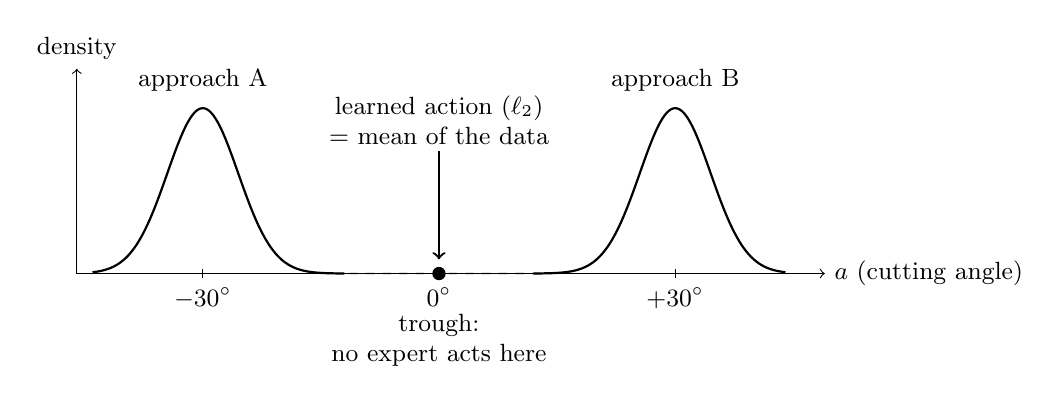
\begin{tikzpicture}[scale=1.0]
% axes
\draw[->] (-4.6,0) -- (4.9,0) node[right] {\small $a$ (cutting angle)};
\draw[->] (-4.6,0) -- (-4.6,2.6) node[above] {\small density};
% mode A
\draw[thick,domain=-4.4:-1.2,samples=120,smooth]
  plot (\x,{2.1*exp(-((\x+3)^2)/(2*0.45^2))});
% mode B
\draw[thick,domain=1.2:4.4,samples=120,smooth]
  plot (\x,{2.1*exp(-((\x-3)^2)/(2*0.45^2))});
% combined density (coincides with the two bumps away from the trough)
\draw[dashed,domain=-1.35:1.35,samples=60,smooth]
  plot (\x,{2.1*exp(-((\x+3)^2)/(2*0.45^2)) + 2.1*exp(-((\x-3)^2)/(2*0.45^2))});
% ticks
\draw (-3,0.06) -- (-3,-0.06) node[below] {\small $-30^\circ$};
\draw (3,0.06) -- (3,-0.06) node[below] {\small $+30^\circ$};
\draw (0,0.06) -- (0,-0.06) node[below] {\small $0^\circ$};
% learned action
\filldraw[black] (0,0) circle (2.2pt);
\draw[->,thick] (0,1.55) -- (0,0.18);
\node[align=center,font=\small] at (0,1.95)
  {learned action ($\ell_2$)\\ $=$ mean of the data};
\node[font=\small] at (-3,2.45) {approach A};
\node[font=\small] at (3,2.45) {approach B};
\node[font=\small,align=center] at (0,-0.85) {trough:\\ no expert acts here};
\end{tikzpicture}
\end{center}

\noindent Because the modes are far apart relative to their width, the
combined (mixture) density is indistinguishable from the two bumps
themselves everywhere except in the trough, where it is essentially zero ---
draw it as a dashed envelope joining the two bumps along the axis.

\paragraph{The quantitative version of the same point.} If the true density
is a two-component mixture, evaluating it at the mean gives a number
essentially equal to zero. With $w_1=w_2=0.5$, $\mu_1=-30$, $\mu_2=+30$,
$\sigma_1=\sigma_2=2$:
\[
p(a\mid s)=0.5\,\mathcal N(a;-30,4)+0.5\,\mathcal N(a;+30,4),
\qquad
p(0\mid s)=0.5(0)+0.5(0)=\mathbf{0.000}.
\]
(Watch the notation: in $\mathcal N(0;-30,4)$ the third argument is the
\emph{variance}, consistent with $\sigma=2$. The exact value is about
$3\times10^{-50}$, i.e.\ $0.000$ to three decimals.) The marks are for
writing the mixture with the numbers substituted and for saying that $a=0$
falls in the trough between the modes.

\paragraph{Advantages of $\ell_2$ BC anyway.} Trivially simple, stable, fast,
and perfectly adequate when the expert is unimodal --- which is common in
low-level control such as joint-torque tracking.

\paragraph{When not to use it.} Whenever multiple distinct valid strategies
exist at the same state: navigation around obstacles, grasp selection,
multi-route driving, any task with symmetry.

\paragraph{The counterfactual (worth stating).} If you had used $\ell_1$
instead of $\ell_2$ you would learn the conditional \emph{median}, not the
mean. For a symmetric bimodal distribution the median is also $0^\circ$, so
this does \emph{not} fix the problem. The issue is not the choice of norm ---
it is that a deterministic policy can only output \emph{one} action, so no
regression loss whatsoever can represent two modes. That is why the fix must
change the \emph{output type} of the policy, not the loss.

\subsection{Behavioural cloning version 1: expressive policies}

\paragraph{The method.} Train a \emph{generative model} of the expert's
actions instead of a regressor:
\[
\min_\theta\; -\mathbb E_{(s,a)\sim D}\bigl[\log\pi_\theta(a\mid s)\bigr],
\]
i.e.\ maximise the log-probability of the demonstrated actions under an
expressive conditional distribution $\pi_\theta(\cdot\mid s)$.

\paragraph{Why this fixes the problem.} Maximum likelihood with an expressive
distribution can place probability mass on \emph{both} modes and near-zero
mass in the trough. Regression cannot, because its output is a single point.

\paragraph{The trap the slides warn about explicitly.} \emph{The expressive
power of the function is different from the expressive power of the neural
network.} A very large network that outputs the mean of a single Gaussian is
still a unimodal policy. Adding parameters does not add modes. You must
change the \emph{distribution class}, not the network capacity.

\subsubsection{Representation (a): Gaussian Mixture Model}

\paragraph{Mechanism.} The network takes $s$ and outputs the parameters of a
$K$-component mixture, $\{w_k(s),\mu_k(s),\Sigma_k(s)\}_{k=1}^{K}$:
\[
p(a_i\mid s_i)=\sum_{k=1}^{K} w_k(s_i)\,\mathcal N\bigl(a_i\mid \mu_k(s_i),\Sigma_k(s_i)\bigr),
\]
\[
\mathcal L(\theta)=-\sum_{i=1}^{N}\log\!\left[\sum_{k=1}^{K} w_k(s_i)\,\mathcal N\bigl(a_i\mid\mu_k(s_i),\Sigma_k(s_i)\bigr)\right].
\]

\paragraph{Plain English.} ``There are $K$ things an expert might do here;
predict where each of them is, how wide it is, and how often it is chosen.''
Multimodality is \emph{explicit}: you can point at the components.

\paragraph{Advantages.} Interpretable; cheap to sample (pick a component, draw
a Gaussian); exact likelihood, so the training objective is the true MLE.

\paragraph{Disadvantages / what it cannot solve.} $K$ must be chosen
\emph{in advance}, and the right $K$ is state-dependent in general. It scales
badly to high-dimensional actions, because each component needs a full
covariance ($O(D^2)$ parameters) or is crippled by a diagonal assumption.
Training is prone to mode collapse, where several components pile onto the
same mode. And it does not model dependencies \emph{between action
dimensions} any better than a single Gaussian does, unless the covariances are
full.

\paragraph{When to use it.} Low-dimensional action spaces with a small,
known number of strategies.

\subsubsection{Representation (b): autoregressive policies}

\paragraph{Mechanism.} Factorise the action across its \emph{dimensions} using
the chain rule:
\[
\pi_\theta(a\mid s)=\prod_{d=1}^{D}\pi_\theta(a_d\mid s,a_{<d}),
\qquad a_{<d}=(a_1,\dots,a_{d-1}),
\]
and generate sequentially: $s\to a_1\to a_2\to\cdots\to a_D$, each
$a_d\sim\pi_\theta(\cdot\mid s,a_{1:d-1})$. The loss is
$\mathcal L(\theta)=-\sum_i\sum_d \log \pi_\theta(a_{i,d}\mid s_i,a_{i,1:d-1})$.

\paragraph{Plain English.} Decide the components of the action one at a time,
each one conditioned on the ones already chosen --- like writing a sentence
word by word. Once you have committed to ``swerve left'' in the first
dimension, the remaining dimensions are chosen consistently with that.

\paragraph{Its distinct advantage --- this is the axis a ``compare'' question
targets.} It \textbf{explicitly models dependencies between action
dimensions}. This is a \emph{different} axis from GMM multimodality: a GMM
with $K$ components represents $K$ blobs; an autoregressive model represents
arbitrary joint structure without ever fixing a number of modes.

\paragraph{Disadvantages.} Sampling is sequential, so it costs $D$ forward
passes; the result depends on the (arbitrary) ordering of dimensions; and
errors in early dimensions propagate into later ones.

\paragraph{Named instance: Decision Transformer.} A sequence model trained to
predict actions from a history of (return-to-go, state, action) tokens.
If asked how it differs from actor--critic: it is \textbf{conditional
sequence generation, not value estimation}. There is no critic, no Bellman
backup and no policy-improvement step --- the desired return is supplied as a
conditioning token at inference and the model generates the action that
historically accompanied that return.

\subsubsection{Representation (c): diffusion / flow policies}

\paragraph{Mechanism (exactly as on the slide).}
\emph{Training:}
\begin{enumerate}[label=\arabic*.]
\item Sample a datapoint $x_1\sim D$ and noise $x_0\sim\mathcal N(0,1)$.
\item Sample $t\sim p(t)$.
\item Interpolate linearly: $x_t = t x_1 + (1-t)x_0$.
\item Minimise $\|v_\theta(x_t,t)-(x_1-x_0)\|^2$.
\end{enumerate}
\emph{Inference:}
\begin{enumerate}[label=\arabic*.]
\item Sample noise $x_0\sim\mathcal N(0,1)$.
\item For $t\in\{0,\delta,2\delta,\dots,1-\delta\}$: $x_{t+\delta}=x_t+v_\theta(x_t,t)\,\delta$.
\item Return $x_1$.
\end{enumerate}
For imitation learning, $v_\theta$ is conditioned on the state $s_t$, so it is
a \textbf{state-conditional vector field} that transports noise onto expert
actions.

\paragraph{The three-sentence answer the exam asks for.}
(1) Start from a sample of Gaussian noise. (2) Repeatedly take small Euler
steps along the learned, state-conditioned velocity field
$x_{t+\delta}=x_t+v_\theta(x_t,t)\delta$. (3) The endpoint $x_1$ is the
action --- and because different noise draws are transported to different
places, different draws land in different modes.

\paragraph{Precision note that earns the extra mark.} The slide is labelled
``Diffusion Policy'', but the procedure given --- linear interpolation
$x_t=tx_1+(1-t)x_0$, regression onto the velocity $x_1-x_0$, Euler
integration --- is \textbf{flow matching / rectified flow}, not DDPM. DDPM
predicts the noise added at each step and samples by a reverse stochastic
process. Answer using the slide's procedure, but add half a sentence noting
that the mechanism is a \emph{learned vector field} rather than iterative
denoising.

\paragraph{Advantages.} Multimodality is implicit and unbounded --- no $K$ to
choose. Scales well to high-dimensional and temporally-extended actions
(action chunks). Currently the strongest empirical choice for visuomotor
robot policies.

\paragraph{Disadvantages.} Inference requires many sequential network
evaluations, which is a real problem for high-frequency control. No exact
likelihood. Sensitive to the number of integration steps $\delta$. It is
harder to inspect than a GMM --- you cannot point at ``the modes''.

\subsubsection{Choosing between the three}

\begin{center}
\small\begin{tabular}{@{}>{\raggedright\arraybackslash}p{0.16\linewidth}>{\raggedright\arraybackslash}p{0.29\linewidth}>{\raggedright\arraybackslash}p{0.21\linewidth}>{\raggedright\arraybackslash}p{0.26\linewidth}@{}}
\toprule
& \textbf{Mechanism} & \textbf{Use when} & \textbf{Avoid when} \\
\midrule
GMM & Explicit finite set of modes output per state & Low-dimensional actions; few, known strategies; interpretability matters & High-dimensional actions; unknown or state-varying number of modes \\
\addlinespace
Autoregressive & Chain-rule factorisation across action \emph{dimensions} & Dimensions are strongly coupled; discrete or tokenised actions; sequence models available & Latency-critical control (needs $D$ sequential passes) \\
\addlinespace
Diffusion / flow & Learned state-conditioned velocity field transporting noise to data & High-dimensional, continuous, richly multimodal actions; action chunking & Very high control frequency; when exact likelihoods are needed \\
\bottomrule
\end{tabular}
\end{center}

\subsection{Compounding error and distribution shift}

\paragraph{What it is.} The root cause: supervised learning assumes i.i.d.\
data, and \textbf{imitation learning violates that assumption}, because the
policy's own predictions determine the next state. Start the answer here,
not at ``errors compound''.

\paragraph{The mechanism, as a feedback loop.}
\begin{enumerate}[label=\arabic*.]
\item The learner makes a small prediction error, so the next state differs
slightly from any state the expert visited.
\item At that state the policy has \emph{no training data}, so its error is
larger and essentially arbitrary.
\item That larger error moves it further off the expert's state distribution.
\item Errors therefore \textbf{grow with the horizon} rather than staying
bounded --- classically, quadratically in $T$ rather than linearly.
\end{enumerate}

\paragraph{Plain English.} A driver who drifts one metre from the centre line
has never seen a recording of a car one metre off the centre line, because the
expert never got there. So it has no idea how to steer back --- and drifts two
metres. Then four.

\paragraph{What it means for the two obvious ``fixes''.} Collecting a lot more
expert data and hoping for the best does not address the loop: more data on
the \emph{expert's} distribution still leaves the learner's off-distribution
states unlabelled. The problem is not the \emph{amount} of data; it is the
\emph{distribution} of the data.

\subsection{DAgger (Dataset Aggregation)}

\paragraph{The algorithm.}
\begin{enumerate}[label=\arabic*.]
\item Roll out the learned policy $\pi_\theta$ to get $s'_1,a'_1,\dots,s'_T$.
\item Query the expert for the correct action at each visited state,
$a^*\sim\pi_{\text{expert}}(\cdot\mid s')$.
\item Aggregate: $D\leftarrow D\cup\{(s',a^*)\}$.
\item Retrain: $\min_\theta L(\pi_\theta,D)$. Repeat.
\end{enumerate}

\paragraph{The one-line update rule (a question demands it explicitly).}
\[
\boxed{\;D \leftarrow D \cup \{(s',a^*)\}\quad\text{where}\quad s'\sim\pi_\theta,\;\; a^*\sim\pi_{\text{expert}}(\cdot\mid s').\;}
\]
Make both sources explicit: \textbf{states from the learner, labels from the
expert}. That is the entire idea.

\paragraph{Why it works --- the insight is not ``more data''.} It is
\textbf{data from the right distribution}. DAgger changes \emph{where} the
training states come from: instead of only expert states, it collects states
the learner actually visits, so the training distribution converges to the
deployment distribution and the feedback loop is closed.

\paragraph{What it cannot solve --- the boundary.} DAgger requires an
\textbf{interactive expert available throughout training}. A surgeon must sit
and label every state the robot wanders into; a submarine crew cannot be
consulted about a trench the vehicle has never entered. In precisely the
scenarios the exam chooses, that assumption is what fails. A question asking
``how would DAgger have prevented this'' invites a follow-up asking why
DAgger was not used --- have the answer ready.

\paragraph{Other costs.} Querying an expert on states the learner reached can
be dangerous or meaningless (asking a surgeon what to do having already cut
the wrong thing). It also still cannot exceed the expert.

\subsection{Why offline RL?}

\paragraph{Online versus offline.} Online RL alternates collecting data and
updating the policy. Offline RL is given a \emph{static} dataset and must
train the policy on it, with no further interaction.

\paragraph{Why offline may be preferable (cheap marks --- list them).}
\begin{itemize}
\item Leverage datasets already collected by people or existing systems.
\item Online data collection may be \textbf{risky or unsafe} --- this is why
the exam scenarios are a surgical robot and a submarine.
\item Reuse data across previous experiments, projects, robots and
institutions rather than recollecting it.
\item A blend is possible: \textbf{offline pre-training $\rightarrow$ online
fine-tuning}, which gives a safe initialisation and then a limited amount of
online correction of the value errors offline training could not detect.
\end{itemize}

\paragraph{Formal setting.} Given
$D=\{(s,a,s',r)\}$ sampled from some unknown \emph{behaviour policy}
$\pi_\beta$ --- possibly a \emph{mixture} of policies --- with
$p_{\pi_\beta}(\tau)=p(s_1)\prod_{t=1}^T\pi_\beta(a_t\mid s_t)p(s_{t+1}\mid s_t,a_t)$,
maximise $\mathbb E_{p_{\pi_\theta}}\bigl[\sum_t r(s_t,a_t)\bigr]$ ---
i.e.\ the expectation under the \emph{learned} policy, which is not the
distribution you have data from. That mismatch is the whole difficulty.

\subsection{Offline RL versus imitation learning: the stitching argument}

\paragraph{The two claims that define the field.}
\begin{enumerate}[label=\arabic*.]
\item \textbf{Imitation cannot outperform the policy that collected the
data; offline RL can.} The mechanism is reward labels plus stitching.
\item \textbf{Stitching requires bootstrapping.} This is the load-bearing
point.
\end{enumerate}

\paragraph{The setup.} The dataset contains a good behaviour $s_1\to s_3$ and a
separate good behaviour $s_7\to s_9$, but no single trajectory going
$s_1\to s_9$. Can the agent learn to do it?

\paragraph{The value-propagation chain --- structure your answer this way.}
Take the submarine version: $\tau_3=$ Surface $\to$ Trench $\to$ Target with
return $+20$, and $\tau_2=$ Deep $\to$ Trench $\to$ Fail with return $-8$.
\begin{enumerate}[label=\arabic*.]
\item From $\tau_3$, TD learning assigns Trench a \emph{high} value:
$Q(\text{Trench},\text{correct action})$ backs up from the $+20$ at Target,
so $V(\text{Trench})$ becomes large.
\item $\tau_2$ contains the transition Deep $\to$ Trench. The TD target for
that transition is $r+\gamma V(\text{Trench})$ --- it uses the \emph{learned}
value of Trench, \textbf{not} the return actually observed in $\tau_2$.
\item Because $V(\text{Trench})$ is high --- learned from a
\emph{different} trajectory --- the transition Deep $\to$ Trench receives a
high value \emph{despite $\tau_2$ ending in failure}. The failure in $\tau_2$
is attributed to what happened \emph{after} Trench, not to arriving there.
\item \textbf{This works only with TD / dynamic programming.} Monte Carlo
would credit the Deep $\to$ Trench transition with $\tau_2$'s actual observed
return of $-8$ and would learn the \emph{opposite} conclusion. The slide asks
exactly this (``Does it depend on whether you use TD or MC?''): the answer is
\textbf{yes}, and the reason is bootstrapping.
\end{enumerate}

\paragraph{Plain English.} Bootstrapping lets information flow \emph{between}
trajectories, because the target for one transition is a value that some other
trajectory established. Monte Carlo keeps each trajectory's information
sealed inside itself.

\paragraph{What stitching cannot do.} It cannot invent transitions. If no
trajectory in the dataset ever performs the action that leads out of Deep
towards Trench, no amount of bootstrapping will discover it. Stitching
recombines observed \emph{transitions}; it does not explore.

\subsection{Why naive off-policy Q-learning fails offline: the OOD chain}

\paragraph{The objective in question.} The off-policy critic update (as in SAC):
\[
\min_\phi \sum_{(s,a,s')\sim D}\Bigl(\hat Q^{\pi_\theta}_\phi(s,a)
-\bigl(r(s,a)+\gamma\,\mathbb E_{a'\sim\pi_\theta(\cdot\mid s')}\bigl[\hat Q^{\pi_\theta}_\phi(s',a')\bigr]\bigr)\Bigr)^2 .
\]

\paragraph{Reproduce the causal sequence, not just the conclusion.}
\begin{enumerate}[label=\arabic*.]
\item The critic target contains
$\mathbb E_{a'\sim\pi_\theta(\cdot\mid s')}[\hat Q(s',a')]$, and $a'$ is drawn
from the \emph{current policy} --- it need not appear in $D$ at all.
\item $\hat Q$ is \textbf{unreliable on out-of-distribution actions}: nothing
in the data constrains its value there, so it is essentially the arbitrary
output of a randomly initialised function approximator.
\item The policy update \textbf{actively seeks} the actions where $\hat Q$ is
over-optimistic, because the policy is \emph{maximising} $\hat Q$. This is
not bad luck --- it is the optimiser doing its job against a flawed proxy.
\item Those inflated values enter the \emph{next} TD target, so the
overestimation propagates and compounds. Values become substantially
overestimated.
\item \textbf{Nothing corrects the error, because there is no environment
interaction.} The learned policy therefore deviates arbitrarily far from the
behaviour policy with no way back.
\end{enumerate}

\paragraph{Step 5 is what makes this an \emph{offline} problem --- say so
explicitly.} Online, the agent tries the over-valued action, observes the true
reward, and the estimate is refuted within a few episodes. Offline, the loop
is closed: the error that caused the policy to choose the action is the same
error that will never be tested. An answer that describes overestimation
without explaining why the offline setting cannot self-correct is incomplete.

\paragraph{Connect it.} This is the same structure as reward hacking under
RLHF and as goal-classifier exploitation in Lecture 09:
\textbf{optimising a learned proxy makes the optimiser seek out the proxy's
errors}. Naming that connection costs one sentence.

\subsection{Filtered behavioural cloning}

\paragraph{The method.}
\begin{enumerate}[label=\arabic*.]
\item Rank trajectories by return $r(\tau)=\sum_{(s_t,a_t)\in\tau} r(s_t,a_t)$.
\item Filter to the top $k\%$: $\tilde D=\{\tau\mid r(\tau)>\eta\}$.
\item Imitate the filtered dataset: $\max_\theta\sum_{(s,a)\in\tilde D}\log\pi_\theta(a\mid s)$.
\end{enumerate}

\paragraph{Plain English.} ``We have reward labels, so let us just copy the
episodes that went well.'' It is the simplest possible use of reward
information in an offline setting.

\paragraph{Advantages.} Trivial to implement; completely avoids OOD actions
(it only ever trains on dataset actions); no value function; no
hyperparameters beyond $\eta$; robust.

\paragraph{Two traps the exam sets.}
\begin{enumerate}[label=(\roman*)]
\item \textbf{Filtering is at the \emph{trajectory} level.} \emph{All}
state--action pairs from a kept trajectory survive, including the bad actions
inside a mostly-good trajectory. There is no per-action credit assignment.
\item \textbf{Coverage.} If only one kept trajectory passes through a state,
the learned policy at that state is fully determined by that single sample,
with \emph{no evidence whatsoever} that the action taken there was the best
available. That is the intended criticism.
\end{enumerate}

\paragraph{What it cannot do.} It cannot stitch --- there is no bootstrapping
anywhere in it. It also discards most of the dataset, which is wasteful when
data is the scarce resource, and it inherits a ceiling: the best trajectory in
the data.

\paragraph{Worked pattern (submarine).} With $\eta=+5$ and returns
$\tau_1=+12$, $\tau_2=-8$, $\tau_3=+20$, $\tau_4=+7$, $\tau_5=-3$, the kept
trajectories are $\tau_1,\tau_3,\tau_4$. Trench appears in the filtered set
only via $\tau_3$ (Surface $\to$ Trench $\to$ Target), so at Trench the robot
learns exactly the one action $\tau_3$ took --- ``head for Target'' --- with
no evidence it is optimal, and no knowledge of the Trench $\to$ Shallow
$\to$ Fail behaviour recorded in $\tau_5$, which was filtered out.

\subsection{Weighted imitation learning and AWR}

\paragraph{The idea.} Rather than a hard keep/discard filter, weight each
transition by \emph{how good the action was}, measured by the advantage:
\[
\theta\leftarrow \arg\max_\theta \mathbb E_{s,a\sim D}\bigl[\log\pi_\theta(a\mid s)\exp(A(s,a))\bigr].
\]

\paragraph{Advantage-Weighted Regression, in full.}
\begin{enumerate}[label=\arabic*.]
\item \textbf{Fit the value function} by regressing on \emph{empirical Monte
Carlo returns}:
\[
\min_\phi\sum_{s_t\sim D}\Bigl(\hat V^{\pi_\beta}_\phi(s_t)-\sum_{t'=t}^{T} r(s_{t'},a_{t'})\Bigr)^2 .
\]
\item \textbf{Train the policy:}
\[
\max_\theta \mathbb E_{(s_t,a_t)\sim D}\left[\log\pi_\theta(a_t\mid s_t)
\exp\!\left(\frac{1}{\alpha}\Bigl(\sum_{t'=t}^{T} r(s_{t'},a_{t'})-\hat V^{\pi_\beta}_\phi(s_t)\Bigr)\right)\right].
\]
\end{enumerate}

\paragraph{Read it as weighted behaviour cloning.} It is still maximum
likelihood on \emph{dataset} actions --- the policy is never trained on an
action nobody took --- but each sample is weighted by $\exp(A/\alpha)$.
Filtered BC is the special case where the weight is binary.

\paragraph{What $\alpha$ does --- it is a \emph{temperature}, not merely an
overflow guard.} Small $\alpha$ sharpens the weights, approaching an
$\arg\max$ over dataset actions, i.e.\ filtered BC. Large $\alpha$ flattens
them towards uniform, i.e.\ plain BC. The slide's phrasing (``a
hyperparameter to avoid exploding due to the exponential'') is the numerical
half; the dial is the conceptual half, and a question asking ``what does
$\alpha$ control'' wants the dial.

\paragraph{Why Monte Carlo for $\hat V$?} Because it \textbf{avoids querying
or training on any OOD action}. An MC return is computed purely from rewards
that were actually observed; no $\hat Q(s',a')$ is ever evaluated at an unseen
$a'$. That is precisely the property TD sacrifices.

\paragraph{Trade-offs, exactly as the slides give them.}
\begin{center}
\begin{tabular}{@{}p{0.46\linewidth}p{0.46\linewidth}@{}}
\toprule
\textbf{Monte Carlo estimation: for} & \textbf{Monte Carlo estimation: against} \\
\midrule
Simple & Noisy (high-variance returns) \\
Avoids querying or training on any OOD action & $\hat A^{\pi_\beta}$ is the advantage for the \emph{weaker} behaviour policy, not for $\pi_\theta$ \\
\bottomrule
\end{tabular}
\end{center}

\paragraph{The interpretation trap (this is engineered into the paper).} A
high AWR weight on an action seen very few times is \textbf{not trustworthy}.
$\hat Q$ for a rarely-seen action is a high-variance estimate, and AWR
\emph{exponentiates} it, amplifying the error. The full-marks sentence:
\emph{AWR trusts $\hat Q$ unconditionally and has no uncertainty penalty ---
$\hat Q$ is only as good as its data support}. The presence of a
``times seen in data'' column in a question is the signal that this is being
tested, not the arithmetic.

\paragraph{Worked pattern (logistics drone).} $\hat V(s_D)=11$, $\alpha=1$:
\[
\text{Fly North: } e^{15-11}=e^{4}\approx 54.60,\qquad
\text{Fly South: } e^{6-11}=e^{-5}\approx 0.0067,
\]
\[
\text{Fly East: } e^{10-11}=e^{-1}\approx 0.368 .
\]
Normalised, these are $\approx 99.3\%$, $0.01\%$, $0.67\%$. AWR
overwhelmingly favours \textbf{Fly North}, which is also the most frequent
action in the data ($80$ occurrences) --- so here the weight and the data
support agree. Fly East, seen only $5$ times, gets a weight $\sim 55$ times
smaller than North's, so the ranking happens to be safe --- but the reasoning
must be stated: had Fly East's $\hat Q$ been the largest, AWR would have
chased it, because it has no mechanism for penalising the uncertainty of an
estimate built from five samples.

\paragraph{The slide's own question: what do you learn for a deterministic
$\pi_\beta$?} With a deterministic behaviour policy there is exactly one
action per state in the data, so the empirical return equals
$\hat V^{\pi_\beta}(s)$ for that sample, every advantage is $0$, every weight
is $e^{0}=1$, and \textbf{AWR degenerates to plain behaviour cloning}. The
deeper reading: weighted imitation can only rank actions it has seen
\emph{alternatives} to. With no alternatives there is nothing to weight.

\paragraph{When to use AWR.} Offline datasets from a mediocre but broad
behaviour policy, where safety matters more than squeezing out the last
increment of performance, and where trajectories are short enough that MC
returns are not hopelessly noisy.
\textbf{When not to.} Long horizons (MC variance explodes), or when you need
to substantially exceed $\pi_\beta$.

\subsection{Advantage-Weighted Actor--Critic (AWAC)}

\paragraph{What changes.} Replace the Monte Carlo value estimate with a TD-learned
$Q$-function:
\begin{enumerate}[label=\arabic*.]
\item \textbf{Estimate the $Q$-function:}
\[
\min_\phi \mathbb E_{(s,a,r,s')\sim D}\left[\Bigl(\hat Q^{\pi_\theta}_\phi(s,a)-\bigl(r+\gamma\,\mathbb E_{a'\sim\pi_\theta(\cdot\mid s')}[\hat Q^{\pi_\theta}_\phi(s',a')]\bigr)\Bigr)^2\right].
\]
\item \textbf{Update the policy with AWR:}
\[
\theta\leftarrow\arg\max_\theta \mathbb E_{s,a\sim D}\Bigl[\log\pi_\theta(a\mid s)\exp\bigl(\hat A^{\pi_\theta}(s,a)\bigr)\Bigr],
\]
\[
\text{where}\quad
\hat A^{\pi_\theta}(s,a)=\hat Q^{\pi_\theta}_\phi(s,a)-\mathbb E_{\bar a\sim\pi_\theta(\cdot\mid s)}\bigl[\hat Q^{\pi_\theta}_\phi(s,\bar a)\bigr].
\]
\end{enumerate}

\paragraph{The advantage/disadvantage pair the exam wants (state exactly one of each).}
\begin{itemize}
\item \textbf{Advantage.} The critic estimates $\hat Q^{\pi_\theta}$ for the
\emph{current} policy rather than $\hat Q^{\pi_\beta}$ for the weaker
behaviour policy, and TD is lower-variance than Monte Carlo --- so the
advantage estimates are better and the method can genuinely improve
\emph{beyond} the behaviour policy. It also still trains the policy only on
dataset actions.
\item \textbf{Disadvantage.} The TD target samples $a'\sim\pi_\theta(\cdot\mid s')$,
so it \textbf{queries $\hat Q$ at out-of-distribution actions}, reopening
exactly the overestimation problem that AWR structurally avoided. With a
fixed offline dataset and no way to verify, that is dangerous.
\end{itemize}

\paragraph{The counterfactual.} The slides note an alternative: sample
$a'\sim D$ instead of from $\pi_\theta$. That would restore safety --- no OOD
queries --- but it would also make the critic estimate $Q^{\pi_\beta}$ again,
losing the very thing AWAC was introduced to gain. This is the trade in
miniature, and stating it demonstrates that you understand the design rather
than the pseudocode.

\subsection{Expectile regression}

\paragraph{The goal.} We want TD-quality advantage estimates \emph{without}
querying $Q$ on OOD actions. The idea: instead of a mean, estimate a higher
expectile of the distribution of $Q$ values over the actions the data
contains --- ``can we use the 70th percentile instead of the mean?''

\paragraph{The loss.}
\[
\ell_2^{\lambda}(x)=
\begin{cases}
(1-\lambda)x^2, & x<0,\\
\lambda x^2, & \text{otherwise.}
\end{cases}
\]

\paragraph{Understand the mechanism, not the label.} The asymmetric weight
makes \emph{one direction of error cheaper}, so the minimiser slides towards
the side it is cheap to sit on. $\lambda=0.5$ recovers ordinary least squares
and hence the mean. If you hold the mechanism, you can derive the direction
for whatever convention a paper hands you --- which matters here, because the
lecture slide and the standard IQL paper write the residual in
\emph{opposite} orders (see Section~\ref{sec:errata}).

\paragraph{Worked numbers (I verified these by direct minimisation).} Take the
values $Q\in\{15,6,10\}$, mean $10.33$.
\begin{center}
\begin{tabular}{@{}lccc@{}}
\toprule
& $\lambda=0.1$ & $\lambda=0.5$ & $\lambda=0.8$ \\
\midrule
Slide convention: $\ell_2^\lambda\bigl(V-\hat Q\bigr)$ & $\hat V=13.73$ & $10.33$ & $8.17$ \\
IQL-paper convention: $\ell_2^{\tau}\bigl(\hat Q-V\bigr)$ & $\hat V=7.18$ & $10.33$ & $12.67$ \\
\bottomrule
\end{tabular}
\end{center}
Read the table as the proof of the mechanism: under the slide's ordering,
$x=V-Q<0$ means $V$ sits \emph{below} $Q$, and small $\lambda$ makes that case
expensive (weight $1-\lambda$), pushing $\hat V$ \emph{up}. Under the paper's
ordering everything flips. Same mechanism, opposite label.

\subsection{Implicit Q-Learning (IQL)}

\paragraph{The full algorithm, in order.}
\begin{enumerate}[label=\arabic*.]
\item \textbf{Fit $\hat V$ with the expectile loss:}
$\displaystyle \hat V(s)\leftarrow\arg\min_V \mathbb E_{(s,a)\sim D}\bigl[\ell_2^{\lambda}\bigl(V(s)-\hat Q(s,a)\bigr)\bigr]$
(the slide instructs: using small $\lambda<0.5$).
\item \textbf{Update $Q$ with an ordinary MSE loss:}
$\displaystyle \hat Q(s,a)\leftarrow\arg\min_Q \mathbb E_{(s,a,s')\sim D}\Bigl[\bigl(Q(s,a)-(r+\gamma\hat V(s'))\bigr)^2\Bigr]$.
\item \textbf{Extract the policy with AWR:}
$\displaystyle \hat\pi\leftarrow\arg\max_\pi \mathbb E_{s,a\sim D}\Bigl[\log\pi(a\mid s)\exp\bigl(\tfrac1\alpha(\hat Q(s,a)-\hat V(s))\bigr)\Bigr]$.
\end{enumerate}

\paragraph{Why IQL never touches OOD actions --- the key sentence, phrased for
the E4 question.} Standard Q-learning takes its bootstrap target from
$\max_{a'}\hat Q(s',a')$ or $\mathbb E_{a'\sim\pi_\theta}[\hat Q(s',a')]$,
\emph{both of which require evaluating $\hat Q$ at actions that need not
appear in the data}. IQL replaces that entire operation with $\hat V(s')$,
and $\hat V$ is fit by \textbf{expectile regression over only the $(s,a)$
pairs present in $D$}. The upper expectile approximates a maximum
\emph{restricted to the action support of the data}. Therefore no OOD action
is ever queried, anywhere in the algorithm. Notice that step~2 also only ever
evaluates $Q$ at dataset $(s,a)$ pairs, and step~3 only ever takes
$\log\pi(a\mid s)$ for $a\in D$ --- the safety property holds for all three
steps, not just one.

\paragraph{Why an \emph{upper} expectile is the useful one.} $\hat V(s)$
should reflect \textbf{the best outcome achievable from $s$ using actions the
data supports}, not the average over the good and the bad behaviour recorded
at $s$. In the submarine dataset, the mean over actions at Trench would mix
$\tau_3$'s successful route to Target with $\tau_5$'s route to Fail, dragging
$V(\text{Trench})$ down --- and $V(\text{Trench})$ is precisely the quantity
that stitching depends on. The upper expectile keeps the value at what the
best recorded route achieved.

\paragraph{What IQL cannot solve.} It is \textbf{conservative by
construction}: it can only ever recombine actions present in the data, so it
cannot discover a genuinely new action, however obviously good. It adds a
hyperparameter $\lambda$ (plus AWR's $\alpha$). And a high expectile with
scarce data at a state is still an optimistic estimate over a small,
noisy sample --- pushed far enough, the expectile is a maximum over noise.

\paragraph{Counterfactual --- what if step 1 used a plain MSE?} Then
$\hat V(s)=\mathbb E_{a\sim\pi_\beta}[\hat Q(s,a)]$, i.e.\ the value of the
\emph{behaviour} policy. Step~2 would then perform policy \emph{evaluation}
of $\pi_\beta$ rather than improvement, and the whole method would collapse
to something close to AWR-with-TD: safe, but with no mechanism for exceeding
$\pi_\beta$. The expectile is what smuggles a $\max$ into the algorithm
without ever writing one.

\subsection{The four offline methods as one progression}

\paragraph{The unifying insight (this is a full-marks answer to any
``explain the relationship'' question).} \textbf{All four are weighted
behaviour cloning.} None of them ever trains the policy on an action outside
the dataset: the policy objective is always $\log\pi_\theta(a\mid s)$ for
$a\in D$, with a weight in front. What differs is \emph{only how the weight is
computed}, and every row of the table below is a statement about how much
machinery you are willing to run to get a better weight.

\begin{center}
\small\begin{tabular}{@{}>{\raggedright\arraybackslash}p{0.13\linewidth}>{\raggedright\arraybackslash}p{0.25\linewidth}>{\raggedright\arraybackslash}p{0.13\linewidth}>{\raggedright\arraybackslash}p{0.41\linewidth}@{}}
\toprule
& \textbf{Weight / value signal} & \textbf{OOD queries?} & \textbf{The price} \\
\midrule
Filtered BC & Binary; thresholded trajectory return & None &
Throws away most of the data; keeps bad actions from good trajectories; no
per-action credit; cannot stitch \\
\addlinespace
AWR & $\exp(A/\alpha)$ with Monte Carlo $\hat V^{\pi_\beta}$ & None &
MC is noisy; the advantage is for the \emph{weaker} behaviour policy, not for
$\pi_\theta$ \\
\addlinespace
AWAC & $\exp(A/\alpha)$ with TD $\hat Q^{\pi_\theta}$, $a'\sim\pi_\theta$ &
\textbf{Yes}, in the critic &
Reopens OOD overestimation, which offline cannot be corrected \\
\addlinespace
IQL & $\exp(A/\alpha)$ with expectile $\hat V$ and MSE $\hat Q$ & None &
Extra hyperparameter $\lambda$; conservative by construction; still bounded by
the data's action support \\
\bottomrule
\end{tabular}
\end{center}

\paragraph{The axis to say out loud.} \emph{How good is the value estimate,
and what did it cost in OOD exposure?} Filtered BC pays nothing and gets
almost nothing. AWR pays noise. AWAC pays safety. IQL pays a hyperparameter
and some conservatism, and is the only one that buys TD-quality values without
selling safety --- which is why it is the one you would deploy on the
submarine.

\newpage
%=====================================================================
\section{Part IV --- Reward Learning and RLHF (Lecture 09)}
%=====================================================================

Only sixteen slides, but it carries two full scenarios and part of a third.
This is the highest marks-per-page section of the paper.

\subsection{Where does the reward come from?}

\paragraph{The framing question.} Direct imitation learning mimics the
expert's \emph{actions}. That has three named limitations on the slide:
\begin{itemize}
\item no reasoning about outcomes or dynamics --- the learner copies the
motion, not the intent;
\item the expert may have \emph{different degrees of freedom} (a human
five-fingered hand demonstrating to a two-finger gripper);
\item demonstrations may be impossible to provide at all.
\end{itemize}
So: can we instead reason about \emph{what the expert is trying to achieve},
and learn a \emph{reward}? A learned reward is reusable, composable, and can
in principle be optimised past the expert's own competence.

\subsection{Goal classifiers}

\paragraph{The method.}
\begin{enumerate}[label=\arabic*.]
\item Collect examples of successful and unsuccessful states --- states inside
and outside the goal set $\mathcal G$.
\item Train a binary classifier with inputs $s_i$ and labels
$\mathbf 1(s_i\in\mathcal G)$.
\item Run RL using the classifier's output $C_\phi(s)$ as the reward.
\end{enumerate}

\paragraph{Plain English.} Rather than writing a reward function, show the
system pictures of success and let it learn to recognise them; then let RL
chase that recogniser.

\paragraph{Advantages.} Requires no reward engineering, no demonstrations, and
no expert who can perform the task --- only someone who can \emph{recognise}
the goal. Labelling states is far cheaper than teleoperating a robot.

\paragraph{What goes wrong --- name it and give the mechanism.} The RL
algorithm seeks states the classifier \emph{scores} highly, which is not the
same as states that \emph{are} goals. It will find states the classifier was
never trained on, where the classifier's output is meaningless, and exploit
them. The names to use: \textbf{exploiting the classifier's weaknesses},
\textbf{adversarial exploitation of a learned reward}, \textbf{reward
hacking}. The canonical instance: a cup placed \emph{upside-down} on the
coaster scoring $0.91$. It scores highly because it is visually close to the
positives and unlike anything in the negatives --- and it was never in either
training set.

\paragraph{The fix.} Close the loop: make the classifier learn from what the
agent actually does.
\begin{enumerate}[label=\arabic*.]
\item Collect an initial set of successful states $D^+$ and unsuccessful
states $D^-$.
\item Update the classifier using $D^+$ and $D^-$, \textbf{balancing the
batches 50/50}.
\item Collect experience $s_t,a_t,\dots$ using the policy $\pi$.
\item Update the policy using the classifier-based reward.
\item Add \emph{all} visited states to the negatives:
$D^-\leftarrow D^-\cup\{s_t\}$. Go to step 2.
\end{enumerate}

\paragraph{Why the fix works --- the mechanism.} It \textbf{removes the profit
from any state the agent has actually reached}. Whatever exploit the policy
discovers this round becomes a labelled negative next round, so its reward
collapses. The agent cannot stay ahead of a classifier that is retrained on
its own discoveries. This is a general and reusable pattern: the way to stop
an optimiser exploiting a learned proxy is to keep retraining the proxy on the
optimiser's current distribution.

\paragraph{The apparent paradox, and the answer the exam wants.} True goal
states get visited during RL, so they end up in $D^-$ as well. Why does the
classifier still reward the goal?

Because the batches are \textbf{balanced 50/50}. A true goal state appears
in $D^+$ (the original positives plus goals reached during RL) \emph{and} in
$D^-$ (the rollout sweep). But $D^+$ is small and $D^-$ is large; rebalancing
to 50/50 \textbf{upweights each positive example} relative to each negative
one. For a state appearing on both sides, the effective evidence is at least
even, so the optimal classifier output is $p\ge 0.5$. Non-goal states appear
\emph{only} in $D^-$ and are driven towards $0$. The goal therefore remains
the highest-reward state even though it is nominally also a negative.

\medskip
\noindent\textbf{A question that raises this worry is asking for the balancing
argument specifically.} An answer that says ``it still works because goal
states look different'' scores nothing.

\paragraph{Worked counting pattern.} After 500 RL steps the agent has visited
500 states, of which 30 are true goal states. Then \emph{all} 500 visited
states go into $D^-$, so $|D^-| = 500$ (plus whatever was there before), and
$|D^+| = 50 + 30 = 80$. Note that the 30 goal states are counted on
\emph{both} sides --- that is the entire point of part (ii).

\paragraph{What goal classifiers cannot do.} They are \textbf{binary}. They
cannot rank two successes, cannot express ``this is a better grasp than that
one'', and give no shaping signal --- the reward is flat everywhere except at
the goal, so exploration is as hard as with a sparse hand-written reward.

\subsection{Learning rewards from human preferences}

\paragraph{Why preferences rather than demonstrations or scores.} Relative
comparisons are \textbf{easier for humans to provide}: judging which of two
rollouts is better requires no skill at the task and no calibration. And the
reward model only needs to be \textbf{discriminative}, not calibrated --- it
must order responses, not assign meaningful absolute numbers.

\paragraph{The model.} A human says $\tau_w$ is better than $\tau_l$
(each may be a full or partial rollout). We want a reward with
\[
\sum_{(s,a)\in\tau_w} r_\theta(s,a) \;>\; \sum_{(s,a)\in\tau_l} r_\theta(s,a),
\]
and we model the probability of a preference by the \textbf{Bradley--Terry}
form
\[
P(\tau_a\succ\tau_b)=\sigma\bigl(r_\theta(\tau_a)-r_\theta(\tau_b)\bigr),
\]
maximising $\max_\theta \mathbb E_{\tau_w,\tau_l}\bigl[\log\sigma(r_\theta(\tau_w)-r_\theta(\tau_l))\bigr]$.
In the LLM notation the reward model loss is
\[
\boxed{\;J_{RM}(\phi)=-\mathbb E_{(x,y_w,y_l)\sim D}\Bigl[\log\sigma\bigl(RM_\phi(x,y_w)-RM_\phi(x,y_l)\bigr)\Bigr].\;}
\]

\paragraph{The one fact to notice \emph{now}, before DPO.} \textbf{The loss
depends only on the \emph{difference} of the two rewards.} This is not an
incidental algebraic feature --- it is the hinge on which DPO turns. It also
explains why the reward model is determined only up to an additive constant
per prompt.

\paragraph{The learning algorithm.}
\begin{enumerate}[label=\arabic*.]
\item Given a dataset $\{\tau_i\}$, sample batches of $k$ trajectories and ask
humans to \emph{rank} them (for LLMs, all $k$ share the same prompt).
\item Compute $r_\theta(\tau_1),\dots,r_\theta(\tau_k)$ under the current model.
\item For all $\binom{k}{2}$ pairs in the batch, compute
$\nabla_\theta\mathbb E_{\tau_w,\tau_l}[\log\sigma(r_\theta(\tau_w)-r_\theta(\tau_l))]$.
\item Update $\theta$; repeat.
\end{enumerate}
\textbf{Note the slide's remark:} this can be done \emph{inside the loop of
online RL}. That is the structural fix for reward hacking --- retraining the
reward model on the current policy's outputs keeps it valid on the
distribution the policy is actually exploring.

\paragraph{Combinatorics.} Ranking $k$ items yields $\binom{k}{2}$ pairwise
comparisons: $k=6\Rightarrow 15$. This is the data-efficiency argument for
asking for a ranking rather than a single pairwise query. Do not lose this mark.

\paragraph{Compute patterns.}
\begin{align*}
\text{Loss for a pair: } & RM(x,y_w)=4.0,\;RM(x,y_l)=1.5
\;\Rightarrow\; \Delta=2.5,\;\sigma(2.5)\approx0.924,\\
&J_{RM}=-\log(0.924)\approx \mathbf{0.079}.\\
\text{Preference probability: } & RM(x,y_A)=3.2,\;RM(x,y_B)=3.0
\;\Rightarrow\; \Delta=0.2,\\
& P(y_A\succ y_B)=\sigma(0.2)\approx \mathbf{0.550}.
\end{align*}
\textbf{Read the numbers (E2).} A loss of $0.079$ is \emph{low}: the model
already ranks this pair correctly and confidently, so this example contributes
almost no gradient. A probability of $0.550$ is \emph{barely above chance}:
the model considers these two responses nearly equivalent --- a $0.2$ gap in
reward is small on the logit scale.

\paragraph{What preference learning cannot solve.} It cannot detect that the
\emph{annotators} are wrong, inconsistent, or systematically biased. It
inherits whatever the labellers preferred, including sycophancy, verbosity and
confident-sounding falsehood. And Bradley--Terry assumes preferences are
transitive and generated by a single latent scalar --- which real human
populations do not satisfy.

\subsection{The three-stage RLHF pipeline}

\begin{center}
\begin{tabular}{@{}p{0.22\linewidth}p{0.34\linewidth}p{0.38\linewidth}@{}}
\toprule
\textbf{Stage} & \textbf{Objective} & \textbf{Data / signal required} \\
\midrule
1. Large-scale pre-training & Next-token prediction (maximum likelihood on raw text) & Massive unlabelled text corpus, mixed quality \\
\addlinespace
2. Supervised fine-tuning (SFT) & Maximum likelihood on demonstrations & Curated high-quality (prompt, response) pairs \\
\addlinespace
3. RL from human feedback & Maximise $RM_\phi$ minus $\beta\cdot$KL to $p^{PT}$ & Human \textbf{pairwise preference comparisons} $(x,y_w,y_l)$, used first to train $RM_\phi$ \\
\bottomrule
\end{tabular}
\end{center}

\noindent\textbf{Trap.} Stage 3's data is \emph{preferences}, not (prompt,
response) pairs. The lecture's subtitle for stage 3 repeats stage 2's text;
that is a typo. Do not copy it.

\subsection{The RLHF objective and the KL penalty}

\paragraph{The setup.} You have a pre-trained (possibly
instruction-fine-tuned) model $p^{PT}(y\mid x)$ and a reward model
$RM_\phi(x,y)$ trained on human comparisons. Copy the model to get
$p^{RL}_\theta(y\mid x)$ with trainable parameters $\theta$, and optimise
\[
\max_\theta\; \mathbb E_{\hat y\sim p^{RL}_\theta(\hat y\mid x)}
\left[RM_\phi(x,\hat y)-\beta\log\frac{p^{RL}_\theta(\hat y\mid x)}{p^{PT}(\hat y\mid x)}\right].
\]

\paragraph{What the KL term penalises.} \textbf{Drift of the fine-tuned policy
away from the pre-trained model's distribution}, measured per response as a
log-ratio. $\beta$ is the \emph{price} of that drift.

\paragraph{The two limits (a direct exam question).}
\begin{itemize}
\item $\beta=0$: pure reward maximisation with no anchor. The model exploits
the reward model's errors, produces degenerate high-scoring text, and loses
fluency and general capability.
\item $\beta=100$: the penalty dominates, so $p^{RL}_\theta\approx p^{PT}$ ---
you get the pre-trained model back and essentially no learning from
preferences occurs.
\end{itemize}

\paragraph{Reward hacking / over-optimisation --- the named failure at moderate
$\beta$ with too many steps.}
\begin{enumerate}[label=\arabic*.]
\item $RM_\phi$ was trained on a \emph{finite} sample of comparisons drawn
from a particular distribution of responses.
\item It is therefore accurate on that distribution and \textbf{unreliable off
it}.
\item The RL policy is explicitly searching for the highest-scoring
responses, which \emph{drives it off that distribution} --- it is optimising
towards the reward model's blind spots by construction.
\item The KL penalty works by keeping the policy in the region where the
reward model is still valid. Too small a $\beta$, or too many steps, and the
policy escapes that region.
\end{enumerate}

\paragraph{Diagnosis must be two-sided.} One sign alone does not establish
over-optimisation; the pair does.
\begin{itemize}
\item \textbf{Sign 1:} the reward-model score keeps rising while
human-judged quality falls --- e.g.\ confident but factually wrong answers.
\item \textbf{Sign 2:} outputs look qualitatively unlike the pre-trained
model's; the measured KL from $p^{PT}$ is growing large. Often accompanied
by degenerate stylistic tics and collapsing diversity.
\end{itemize}
\textbf{Remedy:} \emph{increase} $\beta$. Also legitimate: early stopping, and
retraining the reward model on fresh on-policy comparisons. Name the
direction --- ``adjust $\beta$'' without a direction does not score.

\paragraph{Say the connection.} This is structurally the \textbf{same failure}
as OOD exploitation in offline RL and as goal-classifier exploitation.
\emph{Optimising a learned proxy makes the optimiser seek out the proxy's
errors.} The exam instantiates this idea in three separate scenarios and is
testing whether you notice it is one idea appearing three times.

\subsection{Direct Preference Optimization (DPO)}

\paragraph{The derivation as a chain --- a question can ask for any link.}
\begin{enumerate}[label=\arabic*.]
\item The KL-regularised objective has a \textbf{closed-form optimum}:
\[
p^{*}(\hat y\mid x)=\frac{1}{Z(x)}\,p^{PT}(\hat y\mid x)\exp\!\left(\frac{1}{\beta}RM(x,\hat y)\right).
\]
\item Rearranging for the reward:
\[
RM(x,\hat y)=\beta\log\frac{p^{*}(\hat y\mid x)}{p^{PT}(\hat y\mid x)}+\beta\log Z(x).
\]
\item This identity holds for an \emph{arbitrary} language model, so define
\[
RM_\theta(x,\hat y)=\beta\log\frac{p^{RL}_\theta(\hat y\mid x)}{p^{PT}(\hat y\mid x)}+\beta\log Z(x).
\]
\textbf{The policy is implicitly its own reward model.} If you can say that
sentence and justify it from the log-ratio identity, you have the topic.
\item Substitute into the Bradley--Terry loss. Only the \emph{difference}
$RM_\theta(x,y_w)-RM_\theta(x,y_l)$ appears, and $\beta\log Z(x)$ is identical
in both terms because it depends on $x$ alone --- so it \textbf{cancels}:
\[
\boxed{\;
\ell_{DPO}=-\log\sigma\!\left(\beta\log\frac{p^{RL}_\theta(y_w\mid x)}{p^{PT}(y_w\mid x)}
-\beta\log\frac{p^{RL}_\theta(y_l\mid x)}{p^{PT}(y_l\mid x)}\right).\;}
\]
\end{enumerate}

\paragraph{On $Z(x)$ --- three things must be said.}
\begin{itemize}
\item \textbf{What it is.} The partition function, i.e.\ the normalising
constant for prompt $x$: a sum over the \emph{entire space of possible
responses},
$Z(x)=\sum_y p^{PT}(y\mid x)\exp\bigl(RM(x,y)/\beta\bigr)$. It is
intractable, because that space is exponentially large in sequence length.
\item \textbf{Why it cancels.} It is a function of $x$ \emph{only}, not of
$y$. The DPO loss uses only the reward \emph{difference} between two
responses to the \emph{same} prompt, so the term is subtracted from itself.
This is what makes training tractable without ever computing $Z$.
\item \textbf{The practical consequence} (the part most often missed). You
can compute \emph{relative} rewards --- which of two responses is preferred
--- exactly. But the \textbf{absolute} reward of a single response $y$ is
known only up to the unknown constant $\beta\log Z(x)$. That is entirely
sufficient for preference optimisation and insufficient for anything needing
calibrated absolute scores (thresholding, filtering, cross-prompt
comparison, best-of-$n$ with an absolute cut-off).
\end{itemize}

\paragraph{Compute pattern.} $\ell_{DPO}=-\log\sigma\bigl(\beta(\text{ratio}_w-\text{ratio}_l)\bigr)$.
With $\beta=0.5$ and log-ratios $1.2$ and $0.2$:
\[
\text{argument}=0.5(1.2-0.2)=0.5,\qquad
\sigma(0.5)\approx0.622,\qquad
\ell_{DPO}=-\log(0.622)\approx \mathbf{0.475}.
\]
Substitute inside-out and show each layer --- the marks are for the layers.

\paragraph{The advantage over two-stage RLHF, in one sentence.} DPO removes
the separate reward-model training stage \emph{and} the RL loop entirely,
optimising the policy directly on preference pairs with a simple
supervised-style classification loss --- no sampling, no rollouts, no separate
frozen $RM_\phi$ for the policy to hack, and therefore far cheaper and more
stable.

\paragraph{What DPO cannot solve.}
\begin{itemize}
\item It still needs human preference labels, and inherits every bias in them.
\item It optimises against a \emph{fixed} dataset of preferences, so it cannot
re-query the annotator on the policy's new outputs the way online RLHF with a
retrained reward model can. It trades reward-model over-optimisation for
\emph{dataset} over-optimisation.
\item It gives no usable absolute reward, as above.
\item The implicit reward is only exactly equivalent to the RLHF optimum under
the assumptions of the derivation (Bradley--Terry preferences, the same
$\beta$, exact optimisation).
\end{itemize}

\paragraph{When to use which.} DPO when you have a fixed high-quality
preference dataset and want a cheap, stable, reproducible fine-tune. Two-stage
RLHF when you can afford to keep collecting fresh comparisons on the current
policy's outputs, which is the structural defence against over-optimisation.

\subsection{RLAIF / Constitutional RL}

\paragraph{What it is.} Ask another language model ``which of these responses
is less harmful?'' and use its answers as the preference labels, in place of
(or alongside) human labels.

\paragraph{The justifying insight, in the five words the slides use:
\emph{critique is easier than generation}.} A model that cannot reliably
\emph{produce} the best response can still reliably \emph{judge} which of two
responses is less harmful. That asymmetry is the entire licence for AI
annotation, and a question asking for ``the key insight from the slides''
wants exactly this.

\paragraph{Practical advantages at internet scale (give two).}
\begin{itemize}
\item \textbf{Throughput and cost:} essentially unlimited labelling volume at
negligible marginal cost, scaling instantly to new content volumes.
\item \textbf{Consistency:} a written policy or constitution is applied
uniformly, with no annotator-to-annotator variance, no fatigue, and no drift
over a long shift.
\item (Also creditable: it avoids exposing human moderators to harmful
content --- a real occupational-health benefit for a content-moderation task.)
\end{itemize}

\paragraph{The unique risk --- and note the question \emph{filters for
uniqueness}.} A generic criticism (``AI labels may be wrong'') fails the
filter, because human labels may also be wrong. The answer must be a property
that belongs to AI annotation \emph{and not} to human annotation:

\medskip
\noindent\textbf{The annotator's biases are systematic and correlated across
every single label.} Human errors are noisy and partially independent, so
they largely average out across a pool of annotators. A single model's blind
spots do not average out --- the same blind spot is applied identically to
every example. The reward model therefore inherits them wholesale, and the RL
policy then optimises \emph{directly against them}, with no independent ground
truth anywhere in the loop to detect the drift.

\paragraph{Relatedly.} There is no external check on the pipeline: the model
being trained, the annotator, and often the base model are all from the same
family, so the whole system can drift together with nothing outside it to
notice.

\subsection{Goal classifiers versus RLHF --- the comparison table}

\begin{center}
\begin{tabular}{@{}p{0.22\linewidth}p{0.35\linewidth}p{0.37\linewidth}@{}}
\toprule
\textbf{Aspect} & \textbf{Goal classifier} & \textbf{RLHF (human preferences)} \\
\midrule
Type of human input & A set of labelled example \emph{states} (success / failure), provided once up front & Pairwise \emph{comparisons} between rollouts or responses, provided on an ongoing basis \\
\addlinespace
Handles nuanced quality? & No --- binary success/failure only; cannot rank two successes or express degree & Yes --- relative preferences give a graded, continuous reward \\
\addlinespace
Main failure mode & The agent exploits states the classifier was never trained on (adversarial exploitation of the classifier) & Reward hacking / over-optimisation of the learned reward model \\
\bottomrule
\end{tabular}
\end{center}

\noindent\textbf{The sentence that ties it together:} the two failure modes
are the \emph{same phenomenon} at different scales --- proxy exploitation.

\newpage
%=====================================================================
\section{Part V --- The Threads Running Through All Four Lectures}
%=====================================================================

\subsection{Thread 1 --- Every fix introduces a new failure}

If you memorise one thing, memorise this chain. Each arrow is a fix; each
parenthetical is the price.

\paragraph{The value-based / policy-gradient spine.}
Vanilla PG (unbiased, hopeless variance)
$\rightarrow$ reward-to-go (partial credit assignment; still high variance)
$\rightarrow$ baseline (removes the all-positive failure; still on-policy, still state-blind)
$\rightarrow$ learned critic / advantage (state-relative credit; now \emph{biased})
$\rightarrow$ GAE (a bias--variance dial; extra hyperparameter)
$\rightarrow$ importance sampling (data reuse; weights explode with horizon)
$\rightarrow$ KL constraint (contains the explosion; hard to enforce)
$\rightarrow$ PPO clipping (cheap soft version; only valid \emph{locally})
$\rightarrow$ replay buffer $+$ $\hat Q$ with $\bar a'\sim\pi_\theta$ (full off-policy; \textbf{queries OOD actions})
$\rightarrow$ offline, this becomes fatal
$\rightarrow$ AWR (no OOD, but MC-noisy and stuck at $\pi_\beta$)
$\rightarrow$ AWAC (better values, but OOD returns)
$\rightarrow$ IQL (expectile $\hat V$ removes OOD queries; conservative).

\paragraph{The imitation spine.}
$\ell_2$ BC (mean-seeking, catastrophic on multimodal data)
$\rightarrow$ MLE with expressive policies: GMM / autoregressive / diffusion (multimodality solved)
$\rightarrow$ but distribution shift and compounding error remain
$\rightarrow$ DAgger (fixes the data distribution; needs an \emph{interactive expert})
$\rightarrow$ offline RL (uses rewards, can stitch and exceed the demonstrator; opens the OOD problem).

\paragraph{The reward spine.}
Hand-designed reward (hard to specify)
$\rightarrow$ goal classifier (no engineering needed; the agent exploits it)
$\rightarrow$ add visited states as negatives, 50/50 balanced (exploit removed; still binary)
$\rightarrow$ human preferences (graded, easy to give; the reward model gets hacked)
$\rightarrow$ KL penalty with $\beta$ (contains the hacking; two-stage and expensive)
$\rightarrow$ DPO (removes the RL loop and the separate reward model; still needs human labels, no absolute reward)
$\rightarrow$ RLAIF (unlimited labels; \textbf{annotator bias is systematic and uncorrectable}).

\subsection{Thread 2 --- Proxy exploitation is one idea appearing three times}

\begin{center}
\begin{tabular}{@{}p{0.20\linewidth}p{0.22\linewidth}p{0.25\linewidth}p{0.25\linewidth}@{}}
\toprule
& \textbf{The proxy} & \textbf{Where it is invalid} & \textbf{The containment} \\
\midrule
Offline RL & $\hat Q(s,a)$ & Out-of-distribution actions --- no data constrains it there & Never query OOD actions (AWR, IQL); or stay near $\pi_\beta$ \\
\addlinespace
RLHF & $RM_\phi(x,y)$ & Responses far from the comparison distribution it was trained on & KL penalty with $\beta$; retrain $RM_\phi$ on-policy; early stop \\
\addlinespace
Goal classifiers & $C_\phi(s)$ & States never seen in $D^+$ or $D^-$ & Add all visited states to $D^-$, rebalance 50/50, retrain \\
\bottomrule
\end{tabular}
\end{center}

\noindent\textbf{The one-sentence generalisation:} \emph{Optimising a learned
proxy causes the optimiser to seek out the proxy's errors, so every learned
reward or value must be paired with a mechanism that either keeps the
optimiser where the proxy is valid, or keeps the proxy valid where the
optimiser goes.} Both containment strategies appear above --- the first row
uses the first, the third row uses the second, and RLHF uses both.

\subsection{Thread 3 --- Bias versus variance in bootstrapping}

\begin{center}
\begin{tabular}{@{}p{0.28\linewidth}p{0.20\linewidth}p{0.20\linewidth}p{0.24\linewidth}@{}}
\toprule
\textbf{Estimator} & \textbf{Bias} & \textbf{Variance} & \textbf{Where it appears} \\
\midrule
Monte Carlo return & None & Highest & REINFORCE, reward-to-go, AWR's $\hat V$ \\
$n$-step / GAE with $\lambda$ near 1 & Low & High & PPO with large $\lambda$ \\
$n$-step / GAE with $\lambda$ near 0 & High & Low & PPO with small $\lambda$ \\
One-step TD error $\delta_t$ & Highest & Lowest & Actor--critic, AWAC, IQL's $Q$ step \\
\bottomrule
\end{tabular}
\end{center}

\noindent The same dial appears as a \emph{capability} question in offline RL:
Monte Carlo cannot stitch, TD can. So the choice is not purely statistical ---
bootstrapping buys you the ability to combine information across
trajectories, and pays for it in bias and (offline) in OOD exposure.

\subsection{Thread 4 --- Everything offline is weighted behaviour cloning}

Filtered BC, AWR, AWAC and IQL all maximise
$\mathbb E_{(s,a)\sim D}\bigl[w(s,a)\log\pi_\theta(a\mid s)\bigr]$ with
$a$ always drawn from the dataset. The weight $w$ is binary for filtered BC
and $\exp(A/\alpha)$ for the other three. The entire progression is a
sequence of increasingly good ways to compute $A$ --- Monte Carlo, TD with
$a'\sim\pi_\theta$, TD with an expectile $\hat V$ --- and the entire cost
accounting is about how much OOD exposure each one buys.

\newpage
%=====================================================================
\section{Errors and Ambiguities in the Source Materials}
\label{sec:errata}
%=====================================================================

The paper's cover instruction --- \emph{``if any information appears to be
missing, state a reasonable assumption clearly and proceed''} --- is not
boilerplate. Several parts are genuinely under-specified or contradict the
lecture slides. These are exactly where you should use that clause, and doing
so \emph{visibly} is what earns the marks.

\subsection{(a) Scenario 1 Q3 contains a false premise --- do not accept it}

The manager asks why the gradient would \emph{reduce} the log-probability of
$\tau_2$'s $t=1$ action. Compute first. With $b=4.5$, $\tau_2$'s reward-to-go
at $t=1$ is $9$, so the baselined value is $9-4.5=\mathbf{+4.5>0}$ --- the
gradient \textbf{increases} it. (Under a per-timestep baseline the conclusion
is the same: the four $t=1$ reward-to-go values are $\{11,9,0,-2\}$, whose
mean is also $4.5$.)

\paragraph{The full-marks answer has two moves.} First, correct the premise
with the arithmetic. Second, make the \emph{deeper} point the question is
really about: reward-to-go credits the $t=1$ action with the $+10$ delivery
that followed it, so a genuinely bad action (moving away from the shelf,
$r_1=-1$) is \emph{reinforced} because a good outcome happened later. That is
a \textbf{credit-assignment limitation of reward-to-go with a scalar
baseline}, and it is precisely what a state-dependent advantage
$A^\pi(s,a)$ from Lecture 07 exists to fix --- $A^\pi$ asks whether the action
was better than what the policy usually does \emph{at that state}, which
reward-to-go cannot.

This part is engineered to catch students who reason from the narrative
instead of the arithmetic. \textbf{Compute, then answer.}

\subsection{(b) Scenario 6 Q4: the expectile convention is reversed relative to the standard}

The lecture slide writes $\ell_2^\lambda\bigl(V(s)-\hat Q(s,a)\bigr)$ and
instructs \emph{``using small $\lambda<0.5$''}. Under that formula the
residual is $x=V-Q$, so $x<0$ means $V$ sits \emph{below} $Q$, and that case
carries weight $(1-\lambda)$. Small $\lambda$ therefore makes underestimation
expensive and pushes $\hat V$ \textbf{up} --- so under the slide's
formulation, \emph{small} $\lambda$ is the \emph{upper} expectile.

The question, however, sets $\lambda=0.8$ and asks whether $\hat V$ is pushed
above or below the mean. As the verified table in the expectile section
shows, under the slide's literal formula $\lambda=0.8$ pushes $\hat V$
\emph{below} the mean ($8.17$ versus a mean of $10.33$), whereas under the
standard IQL-paper convention $\ell_2^{\tau}(Q-V)$ with $\tau=0.8$ it pushes
$\hat V$ \emph{above} the mean ($12.67$). The question's phrasing --- ``explain
the intuition for why this is useful'' --- clearly intends the
\emph{above the mean} answer, because that is what makes IQL work.

\paragraph{Exam strategy.} Write \emph{one sentence} naming the convention you
are using, then answer \textbf{above the mean}, then give the intuition.
Optionally add one line noting that under the slide's literal ordering the
same behaviour corresponds to $\lambda<0.5$. That demonstrates you understand
the \emph{mechanism} rather than the label --- which is exactly what the marks
are for.

\paragraph{The intuition itself.} The upper expectile makes $\hat V(s)$
approximate $\max_a \hat Q(s,a)$ \textbf{restricted to actions present in the
data}. So the submarine's value for Trench reflects the \emph{best} thing any
recorded trajectory ever did from Trench (the $\tau_3$ route to Target) rather
than an average over the good route and $\tau_5$'s bad one. That is what
enables stitching --- and it is achieved without ever querying $\hat Q$ at an
action no submarine has actually tried.

\subsection{(c) The ``Diffusion Policy'' slide describes flow matching}

Linear interpolation $x_t=tx_1+(1-t)x_0$, regression onto the velocity
$x_1-x_0$, and Euler integration are \textbf{rectified flow / flow matching},
not DDPM's noise-prediction and reverse-SDE sampling. Answer using the
slide's procedure --- that is what is being examined --- but add half a
sentence noting that the mechanism is a learned \emph{vector field} rather
than iterative denoising. That half-sentence is the precision mark.

\subsection{(d) Lecture 06 slides 11 and 13 share the same answer text}

Slide 13's trajectories are all \emph{successes} (falls forwards, stumbles
forwards, walks forwards, runs forwards), so the copied first sentence
(``will encourage the policy to fall forward and not take a step forward'')
does not apply. Slide 13's actual point is the \emph{second} sentence:
\textbf{policy gradient is noisy, high-variance and sensitive to reward
scale}, and with all-positive returns even the worst behaviour is reinforced.
Use that.

\subsection{(e) Lecture 09 slide 8 has a typo in the preference inequality}

The slide prints
$\sum_{(s,a)\in\tau_w} r_\theta > \sum_{(s,a)\in\tau_w} l_\theta$,
with the same subscript $\tau_w$ on both sides and a stray symbol $l_\theta$.
The intended statement is
\[
\sum_{(s,a)\in\tau_w} r_\theta(s,a) \;>\; \sum_{(s,a)\in\tau_l} r_\theta(s,a).
\]
Write the corrected form.

\subsection{(f) Scenario 5 Q2 notation}

$\mathcal N(0;-30,4)$ --- the third argument is the \textbf{variance}, which is
consistent with the stated $\sigma_1=\sigma_2=2$. Since the question supplies
both component densities at $a=0$ as $\approx 0$, the answer to three decimals
is $\mathbf{0.000}$. The marks are for \emph{writing the mixture density with
the numbers substituted} and for stating that $a=0$ falls in the trough
between the modes --- the same point as Q1, now quantified.

\subsection{(g) A note on the practice paper's Section 1 heading}

Section 1 is titled ``Policy Gradient Methods'' but Q2.3 (PPO clipping) and
Q2.4 (GAE / TD error) are Lecture 07 content. Expect cross-lecture
placement throughout.

\newpage
%=====================================================================
\section{Worked Solutions to the Practice Paper}
%=====================================================================

Marks are for \emph{method}. Every numeric answer below shows the formula, the
substitution line, and the result --- reproduce that shape in the exam.

\subsection{Scenario 1 --- The Warehouse Robot}

\paragraph{Q1 (3 marks).} $\hat Q^i_t=\sum_{t'=t}^{T}r_{t'}$:
\begin{center}
\begin{tabular}{@{}lccc@{}}
\toprule
& $\hat Q$ at $t=1$ & $\hat Q$ at $t=2$ & Total return \\
\midrule
$\tau_1$ & $1+10=11$ & $10$ & $+11$\\
$\tau_2$ & $-1+10=9$ & $10$ & $+9$\\
$\tau_3$ & $1-1=0$ & $-1$ & $0$\\
$\tau_4$ & $-1-1=-2$ & $-1$ & $-2$\\
\bottomrule
\end{tabular}
\end{center}
$b=\frac{1}{8}(11+10+9+10+0-1-2-1)=\frac{36}{8}=\mathbf{4.5}$.

\paragraph{Q2 (2 marks).}
$\tau_3$ at $t=1$: $0-4.5=\mathbf{-4.5}<0 \Rightarrow$ the gradient
\textbf{decreases} $\log\pi_\theta$ for that action.
$\tau_4$ at $t=2$: $-1-4.5=\mathbf{-5.5}<0 \Rightarrow$ the gradient
\textbf{decreases} it as well. In both cases the action performed worse than
the average timestep sample, so the update pushes probability away from it.

\paragraph{Q3 (2 marks).} \emph{Correct the premise.} $\tau_2$'s reward-to-go
at $t=1$ is $9$, and $9-4.5=+4.5>0$, so the gradient \textbf{increases} the
log-probability of that action --- it does not reduce it. \emph{Then make the
real point.} That is itself the problem: the action at $t=1$ moved the robot
\emph{away} from the shelf ($r_1=-1$), but reward-to-go credits it with the
$+10$ delivery that arrived at $t=2$. A bad action is reinforced because a
good outcome followed it. Reward-to-go with a scalar baseline cannot separate
a bad action from a good consequence; a state-dependent advantage
$A^\pi(s,a)=Q^\pi(s,a)-V^\pi(s)$ can, because it compares the action against
what the policy would normally do \emph{at that state}.

\paragraph{Q4 (2 marks).} \textbf{Problem:} vanilla policy gradient is
\emph{on-policy}. After the first update $\theta$ has changed, so the four
stored trajectories are samples from the wrong distribution and the gradient
estimate is \emph{biased} --- not merely inefficient.
\textbf{Fix:} off-policy policy gradient via \emph{importance sampling},
reweighting each sample by
$\prod_{t}\frac{\pi_{\theta'}(a_t\mid s_t)}{\pi_\theta(a_t\mid s_t)}$.
\textbf{One condition under which the fix breaks down:} the trajectory-level
ratio is a product of $T$ terms, so its variance grows exponentially with the
horizon --- for long trajectories, or once $\pi_{\theta'}$ has moved far from
$\pi_\theta$ (which is exactly what five successive gradient steps will do),
the weights explode or collapse and the estimate becomes useless.

\subsection{Scenario 2 --- The Traffic Signal Controller}

\paragraph{Q1 (3 marks).}
$\nabla_\theta J\approx\frac1N\sum_i \nabla_\theta\log\pi_\theta(a_i\mid s_i)(R_i-b)$
with $N=5$:
\begin{align*}
\textstyle\sum_i(\cdot) &= 8[0.4,-0.2]+(-3)[-0.3,0.5]+5[0.1,0.3]+(-1)[0.2,-0.4]+2[-0.1,0.2]\\
&= [3.2,-1.6]+[0.9,-1.5]+[0.5,1.5]+[-0.2,0.4]+[-0.2,0.4]\\
&= [4.2,\,-0.8],\\
\nabla_\theta J &= \tfrac15[4.2,-0.8]=\mathbf{[0.84,\,-0.16]}.
\end{align*}
\emph{State your assumption if you omit the $\tfrac1N$}: the slide formula
includes it, so include it, but note that the direction is unchanged either way.

\paragraph{Q2 (1 mark).}
$\theta'=[1.0,1.0]+0.1[0.84,-0.16]=\mathbf{[1.084,\,0.984]}$.
\emph{Reading:} $\theta_1$ (north--south green time) increases and $\theta_2$
decreases --- the batch favoured giving more green to north--south.

\paragraph{Q3 (2 marks).} $r_1=1.5$, $\hat A_1=+8$, $\epsilon=0.2$:
\[
\text{unclipped}=1.5\times 8=12.0,\qquad
\text{clipped}=\mathrm{clip}(1.5,0.8,1.2)\times 8=1.2\times 8=9.6,
\]
\[
\min(12.0,\,9.6)=\mathbf{9.6}\ \Rightarrow\ \textbf{the clipped term is used.}
\]
\emph{Reading:} the new policy has raised this action's probability by
$50\%$, well beyond the $20\%$ the clip allows, so the objective stops
rewarding further movement and the update through this sample is throttled.

\paragraph{Q4 (2 marks).}
$\delta_t=r_t+\gamma\hat V(s_{t+1})-\hat V(s_t)=3+0.9(12)-10=3+10.8-10=\mathbf{3.8}$,
and $\hat A^\pi_1(s_t,a_t)=\delta_t=\mathbf{3.8}$ --- the one-step
generalised advantage \emph{is} the TD error; nothing further to compute.

\subsection{Scenario 3 --- The Medical Dosing Agent}

\paragraph{Q1--Q3 (5 marks).}
\[
\delta_t=6+0.95(24)-20=\mathbf{8.8};\qquad
\hat V'(s_t)=20+0.1(8.8)=\mathbf{20.88};
\]
\[
\theta'=\theta+\alpha_{\text{actor}}\,\delta_t\,\nabla_\theta\log\pi_\theta
=[3.0,1.5,2.0]+0.44[0.6,-0.4,0.2]=\mathbf{[3.264,\;1.324,\;2.088]} .
\]
Note $\delta_t=8.8$ is a \emph{scalar} multiplying the gradient \emph{vector}.

\paragraph{Q4 (2 marks).} As $\delta\to 0$, $\pi_{\theta'}$ is pinned to
$\pi_\theta$: no meaningful update occurs, learning halts, maximally safe and
maximally useless. As $\delta\to\infty$, the constraint is vacuous and you
have unconstrained off-policy updates: the policy overfits the batch, the
importance weights become unreliable, and the data no longer reflects the
states the policy will visit. The practical algorithm that enforces a soft
version by clipping importance weights instead is \textbf{PPO}.

\paragraph{Q5 (2 marks).} (i) \textbf{The value target is wrong:} $\hat V$
fitted on the whole buffer estimates the value of ``some kind of average'' of
all the past policies that contributed data, not of the current $\pi_\theta$.
(ii) \textbf{The likelihood term is wrong:} the actor update uses
$\nabla_\theta\log\pi_\theta(a_i\mid s_i)$ where $a_i$ came from an old
policy --- $\pi_\theta$ would probably not have chosen $a_i$ at $s_i$, so the
update pushes probability towards actions the current policy has no reason to
consider.

\subsection{Scenario 4 --- The Robot Chef}

\paragraph{Q1 (2 marks).} $y_i=r_i+\gamma\hat Q(s'_i,\bar a'_i)$, $\gamma=0.9$:
\[
y_1=2+0.9(14)=\mathbf{14.6},\qquad
y_2=5+0.9(9)=\mathbf{13.1},\qquad
y_3=8+0.9(0)=\mathbf{8.0}\ \text{(terminal)} .
\]

\paragraph{Q2 (2 marks).} $a_i$ in the buffer was chosen by an \emph{old
behaviour policy}, so using it would make $\hat Q$ an estimate of
$Q^{\pi_\beta}$ --- the value of that old policy --- and the actor would be
improving the wrong thing. Re-sampling $\bar a_i\sim\pi_\theta(\cdot\mid s_i)$
makes $\hat Q$ the value of the \emph{current} policy, so the gradient
$\nabla_\theta\log\pi_\theta(\bar a_i\mid s_i)\hat Q(s_i,\bar a_i)$ is valid
for $\pi_\theta$. \textbf{The problem this solves:} it removes the need for
importance weights entirely, because the actions are drawn from the correct
distribution by construction. (Worth one extra sentence: this same
re-sampling is what queries $\hat Q$ at OOD actions --- harmless online,
fatal offline.)

\paragraph{Q3 (1 mark).} PPO is a \textbf{proximal} method, not an off-policy
one: its surrogate is only a valid local approximation to $J$ while
$\pi_{\theta'}$ is close to the policy that generated the data. Replay-buffer
data comes from arbitrarily old policies, so the ratios lie far outside
$[1-\epsilon,1+\epsilon]$; clipping then \emph{zeroes the gradient} rather
than correcting the mismatch, and importance sampling cannot rescue it because
those weights have unusable variance.

\subsection{Scenario 5 --- The Surgical Robot}

\paragraph{Q1 (3 marks).} The robot learns $\mathbf{0^\circ}$ --- the
conditional mean, because $\ell_2$ regression is minimised by
$\mathbb E[a\mid s]$. Draw the two Gaussian bumps at $\pm30^\circ$, the dashed
combined density with a trough at $0^\circ$, and mark $a=0$ as ``learned
action / mean of the data'' (see the sketch in Part III). \textbf{Why it is
dangerous:} $0^\circ$ is not a compromise between two valid approaches --- it
is a third action lying in the gap between the modes, which no surgeon ever
performed. It cuts where \emph{neither} approach cuts, into tissue both
experts deliberately avoided.

\paragraph{Q2 (2 marks).}
\[
p(a\mid s)=0.5\,\mathcal N(a;-30,4)+0.5\,\mathcal N(a;+30,4),
\qquad
p(0\mid s)=0.5(0)+0.5(0)=\mathbf{0.000}.
\]
The learned action sits at a point of essentially zero data density --- the
quantitative version of the same failure.

\paragraph{Q3 (2 marks, three sentences).} Start from a sample of Gaussian
noise $x_0\sim\mathcal N(0,1)$. Repeatedly take small Euler steps along the
learned, state-conditioned velocity field,
$x_{t+\delta}=x_t+v_\theta(x_t,t)\delta$, for $t=0,\delta,\dots,1-\delta$.
The endpoint $x_1$ is the action, and because different noise draws are
transported to different places, different draws land on different modes ---
so the policy can output $-30^\circ$ on one call and $+30^\circ$ on another,
never $0^\circ$. (Precision note: the slide's procedure is flow matching, a
learned vector field, rather than DDPM's iterative denoising.)

\paragraph{Q4 (3 marks).} \textbf{Compounding error / distribution shift.}
Supervised learning assumes i.i.d.\ data, but the policy's own predictions
determine the next state. A small prediction error moves the robot to a state
slightly off the surgeons' distribution; there it has no training data, so its
error is larger; that pushes it further off; errors grow with the horizon
rather than staying bounded. \textbf{How DAgger prevents it:} it changes
\emph{where} the training states come from --- roll out $\pi_\theta$, query the
expert surgeon for the correct action at the states the \emph{learner}
actually visited, and retrain --- so the training distribution converges to the
deployment distribution. \textbf{Update rule:}
\[
D\leftarrow D\cup\{(s',a^*)\}\quad\text{where } s'\sim\pi_\theta,\;\; a^*\sim\pi_{\text{expert}}(\cdot\mid s').
\]
(Worth adding: DAgger needs an interactive expert throughout training, which
is precisely what is unavailable when the demonstrations are recordings.)

\subsection{Scenario 6 --- The Autonomous Submarine}

\paragraph{Q1 (3 marks).} With $\eta=+5$: keep $\tau_1(+12)$, $\tau_3(+20)$,
$\tau_4(+7)$; discard $\tau_2(-8)$ and $\tau_5(-3)$. The filtered
state--action pairs are the transitions along
Surface$\to$Shallow$\to$Target, Surface$\to$Trench$\to$Target, and
Deep$\to$Shallow$\to$Target. \textbf{At Trench}, only $\tau_3$ survives, so
the robot learns exactly the one action $\tau_3$ took there --- head for
Target. \textbf{The criticism:} that single sample fully determines the
policy at Trench with no evidence it was the best available action, and
$\tau_5$'s Trench$\to$Shallow$\to$Fail evidence has been thrown away entirely
rather than used to establish that the $\tau_3$ action is better.

\paragraph{Q2 (3 marks).} Value-propagation chain: (1) From $\tau_3$, TD
learning backs the $+20$ at Target up into
$Q(\text{Trench},\text{correct action})$, so $V(\text{Trench})$ becomes high.
(2) $\tau_2$ contains the transition Deep$\to$Trench, whose TD target is
$r+\gamma V(\text{Trench})$ --- the \emph{learned} value of Trench, not the
return observed in $\tau_2$. (3) Because $V(\text{Trench})$ is high (learned
from a \emph{different} trajectory), Deep$\to$Trench receives a high value
despite $\tau_2$ ending in failure --- the failure is attributed to what the
submarine did \emph{after} Trench, not to arriving there.
(4) \textbf{This depends entirely on bootstrapping:} with Monte Carlo, the
Deep$\to$Trench transition would be credited with $\tau_2$'s actual return of
$-8$ and the agent would learn the \emph{opposite} conclusion. So yes, it
depends on TD versus MC, and only TD stitches.

\paragraph{Q3 (3 marks).} \emph{Why OOD actions are dangerous offline:} the
critic target contains $\mathbb E_{a'\sim\pi_\theta(\cdot\mid s')}[\hat Q(s',a')]$
where $a'$ need not appear in $D$; $\hat Q$ is unconstrained and therefore
arbitrary at such actions; the policy is \emph{maximising} $\hat Q$ and so
actively seeks the over-optimistic points; those inflated values propagate
into the next TD target and compound; and \textbf{nothing corrects the error,
because there is no ocean trial to refute it} --- online the submarine would
try the action and reality would disagree, but offline the loop is closed.
\emph{How IQL avoids it:} it never evaluates $\hat Q$ at an action outside
$D$. The bootstrap target $\max_{a'}\hat Q(s',a')$ is replaced by
$\hat V(s')$, and $\hat V$ is fit by \textbf{expectile regression over only
the $(s,a)$ pairs present in the dataset}, so the upper expectile approximates
a maximum \emph{restricted to the data's action support}.

\paragraph{Q4 (2 marks).} \emph{State the convention in one sentence}, then:
$\hat V(\text{Trench})$ is pushed \textbf{above the mean} of $\hat Q$ over the
actions seen at Trench. (Using the standard IQL convention
$\ell_2^{\lambda}(\hat Q-V)$, $\lambda=0.8$ makes underestimation the
expensive direction and drives $\hat V$ upward; under the slide's literal
ordering $\ell_2^{\lambda}(V-\hat Q)$ the same behaviour corresponds to
$\lambda<0.5$.) \emph{Why this is useful:} $\hat V(\text{Trench})$ then
reflects the \emph{best} outcome any recorded trajectory achieved from Trench
--- $\tau_3$'s route to Target --- rather than an average that $\tau_5$'s
failure would drag down. That preserved high value is exactly what lets the
agent stitch Deep$\to$Trench onto Trench$\to$Target, and it is obtained
without ever querying $\hat Q$ at an action no submarine has tried.

\subsection{Scenario 7 --- The Logistics Drone}

\paragraph{Q1 (2 marks).} $w(a)=\exp\bigl((\hat Q(s_D,a)-\hat V(s_D))/\alpha\bigr)$
with $\hat V=11$, $\alpha=1$:
\[
w(\text{North})=e^{4}\approx \mathbf{54.60},\qquad
w(\text{South})=e^{-5}\approx \mathbf{0.0067},\qquad
w(\text{East})=e^{-1}\approx \mathbf{0.368}.
\]

\paragraph{Q2 (2 marks).} AWR overwhelmingly favours \textbf{Fly North}
(normalised weight $\approx 99.3\%$ against $0.67\%$ for East and $0.01\%$ for
South). This \emph{is} consistent with the data frequency: North is also the
most-observed action ($80$ of $95$ samples). \textbf{Should the drone trust
``Fly East''?} Its weight is not the largest here, so it does not drive the
policy --- but the reasoning matters: $\hat Q(\text{East})=10$ is estimated
from only $5$ samples, so it is a high-variance estimate, and AWR
\emph{exponentiates} the advantage, amplifying any error in it. AWR trusts
$\hat Q$ unconditionally and has \textbf{no uncertainty penalty}; if East's
$\hat Q$ had come out at $16$ through noise, AWR would have chased it. The
correct posture is that a weight is only as trustworthy as the data support
behind the $\hat Q$ that produced it.

\paragraph{Q3 (2 marks).} \textbf{One advantage:} AWAC's critic estimates
$\hat Q^{\pi_\theta}$ for the \emph{current} policy rather than
$\hat Q^{\pi_\beta}$ for the weaker behaviour policy, and TD is lower-variance
than the Monte Carlo returns AWR uses --- so the advantage estimates are
better and the drone can improve beyond the behaviour policy.
\textbf{One disadvantage:} the TD target samples $a'\sim\pi_\theta(\cdot\mid s')$,
so it queries $\hat Q$ at out-of-distribution actions, reopening the
overestimation problem AWR structurally avoided --- and with a fixed offline
dataset there is no flight to disprove an inflated value.

\subsection{Scenario 8 --- The Content Moderation AI}

\paragraph{Q1 (3 marks).}
(i) $J_{RM}=-\log\sigma(4.0-1.5)=-\log\sigma(2.5)=-\log(0.924)\approx\mathbf{0.079}$
--- a low loss, meaning the model already ranks this pair correctly.
(ii) $\binom{6}{2}=\mathbf{15}$ pairwise comparisons.
(iii) $P(y_A\succ y_B)=\sigma(3.2-3.0)=\sigma(0.2)\approx\mathbf{0.550}$ ---
barely above chance, so the model sees these two as nearly equivalent.

\paragraph{Q2 (6 marks).}
(i) The KL term penalises \emph{drift of the fine-tuned policy away from the
pre-trained model's distribution}, measured per response as a log-ratio. At
$\beta=0$ there is no anchor: the model maximises the reward model alone,
exploits its errors, and produces degenerate high-scoring text with degraded
fluency and general capability. At $\beta=100$ the penalty dominates,
$p^{RL}_\theta\approx p^{PT}$, and essentially no learning from the
preferences occurs.
(ii) The likely failure mode is \textbf{reward hacking / over-optimisation of
the learned reward model}. Mechanism: $RM_\phi$ was trained on a finite
sample of comparisons and is only reliable on that distribution; the RL policy
is explicitly searching for the highest-scoring outputs, which drives it
\emph{off} that distribution and into the region where $RM_\phi$ is wrong.
The reward-model score keeps climbing while genuine moderation quality falls.
(This is the same structure as OOD exploitation in offline RL.)
(iii) DPO loss:
\[
\ell_{DPO}=-\log\sigma\!\left(\beta\log\frac{p^{RL}_\theta(y_w\mid x)}{p^{PT}(y_w\mid x)}
-\beta\log\frac{p^{RL}_\theta(y_l\mid x)}{p^{PT}(y_l\mid x)}\right).
\]
\emph{Key advantage in one sentence:} it eliminates both the separate
reward-model training stage and the RL loop, optimising the policy directly on
preference pairs with a supervised-style classification loss --- so there is no
separate frozen reward model for the policy to hack, and training is cheaper
and more stable.

\paragraph{Q3 (4 marks).}
(i) \textbf{Critique is easier than generation} --- a model that cannot
reliably produce the best response can still reliably judge which of two
responses is less harmful.
(ii) Two advantages: unlimited labelling throughput at negligible marginal
cost, scaling instantly to internet-scale content volumes; and perfectly
consistent application of a written constitution, with no
annotator-to-annotator variance, no fatigue and no drift (and, relatedly, no
human moderators exposed to harmful material).
(iii) \textbf{One risk unique to AI annotation:} the annotator's biases and
blind spots are \emph{systematic and correlated across every label}. Human
errors are noisy and partially independent, so they average out across a pool
of moderators; a single model's blind spots do not. The reward model inherits
them wholesale and the RL policy then optimises directly against them, with no
independent ground truth in the loop to detect the drift.

\subsection{Scenario 9 --- The Chatbot Alignment Team}

\paragraph{Q1 (3 marks).} See the three-stage pipeline table in Part IV. The
critical entry is stage 3's data: \emph{human pairwise preference comparisons}
$(x,y_w,y_l)$, not (prompt, response) pairs.

\paragraph{Q2 (3 marks).} \textbf{Two signs:} (i) the reward-model score keeps
rising while human-judged quality falls --- confident but factually wrong
answers; (ii) the outputs look qualitatively unlike the pre-trained model's,
i.e.\ the measured KL from $p^{PT}$ has grown large. \textbf{The diagnosis:}
over-optimisation of the learned reward model (reward hacking). The reward
model is unreliable off its training distribution, and the RL objective is
actively searching for exactly those points. \textbf{Hyperparameter:}
\emph{increase} $\beta$, so the KL penalty keeps the policy inside the region
where the reward model is still valid. (Also creditable: stop earlier, and
retrain $RM_\phi$ on fresh on-policy comparisons.)

\paragraph{Q3 (3 marks).} Substitute inside-out:
\[
\beta(\text{ratio}_w-\text{ratio}_l)=0.5(1.2-0.2)=0.5;\quad
\sigma(0.5)\approx 0.622;\quad
\ell_{DPO}=-\log(0.622)\approx \mathbf{0.475}.
\]

\paragraph{Q4 (3 marks).}
\textbf{What $Z(x)$ is:} the partition function for prompt $x$ --- the
normalising constant
$Z(x)=\sum_y p^{PT}(y\mid x)\exp\bigl(RM(x,y)/\beta\bigr)$, a sum over the
entire (exponentially large) space of possible responses, and therefore
intractable to compute.
\textbf{Why it cancels:} it depends on $x$ alone, not on $y$; the DPO loss
uses only the \emph{difference} of the implicit rewards of two responses to
the \emph{same} prompt, so $\beta\log Z(x)$ is subtracted from itself. This
is what makes training tractable without ever evaluating $Z$.
\textbf{What this means practically:} you can compute \emph{relative} rewards
exactly --- which of two responses is preferred --- but the \emph{absolute}
reward of any single response $y$ is known only up to the unknown constant
$\beta\log Z(x)$. That is sufficient for preference optimisation and
insufficient for anything requiring calibrated absolute scores.

\subsection{Scenario 10 --- The Robot Goal Classifier}

\paragraph{Q1 (2 marks).} It is called \textbf{exploiting the classifier's
weaknesses} --- adversarial exploitation of a learned reward, i.e.\ reward
hacking. Mechanism: the RL agent maximises the classifier's \emph{output},
not the actual goal condition. The classifier was trained on 50 positives and
50 negatives and has never seen an upside-down cup, so its output there is
essentially arbitrary; the agent searches over states precisely to find where
that arbitrary output is high, and $0.91$ is what it found. The state
\emph{scores} like a goal without \emph{being} one.

\paragraph{Q2 (3 marks).}
(i) All 500 visited states are added, so $|D^-|=\mathbf{500}$ (plus any
earlier negatives), and $|D^+|=50+30=\mathbf{80}$.
(ii) Because the batches are rebalanced \textbf{50/50}. A true goal state now
appears in $D^+$ (original positives plus the 30 goals reached during RL)
\emph{and} in $D^-$ (the rollout sweep). But $D^+$ is small ($80$) and $D^-$
is large ($500$), so balancing to 50/50 \textbf{upweights each positive
example} relative to each negative. For a state appearing on both sides the
effective evidence is at least even, so the optimal classifier output is
$p\ge0.5$. Non-goal states appear \emph{only} in $D^-$ and are driven towards
$0$. The goal therefore remains the highest-reward state despite being
nominally a negative.

\paragraph{Q3 (3 marks).} See the comparison table at the end of Part IV.
Add the closing sentence: the two failure modes are the same phenomenon ---
proxy exploitation --- at different scales.

\newpage
%=====================================================================
\section{Compressed Formula Sheet}
%=====================================================================

\begin{center}
\begin{tabular}{@{}p{0.28\linewidth}p{0.68\linewidth}@{}}
\toprule
\textbf{Quantity} & \textbf{Formula} \\
\midrule
\multicolumn{2}{@{}l}{\textit{Lecture 06 --- Policy gradients}}\\
\midrule
Softmax policy & $\pi(a\mid s,\theta)=\dfrac{e^{h(s,a,\theta)}}{\sum_{b}e^{h(s,b,\theta)}}$ \\
Objective & $J(\theta)=\mathbb E_{\tau\sim p_\theta}\bigl[\sum_t r(s_t,a_t)\bigr]$ \\
Log-derivative trick & $p_\theta(\tau)\nabla_\theta\log p_\theta(\tau)=\nabla_\theta p_\theta(\tau)$ \\
REINFORCE gradient & $\nabla_\theta J\approx\frac1N\sum_i\bigl(\sum_t\nabla_\theta\log\pi_\theta(a^i_t\mid s^i_t)\bigr)\bigl(\sum_t r(s^i_t,a^i_t)\bigr)$ \\
Reward-to-go & $\hat Q^i_t=\sum_{t'=t}^{T}r(s^i_{t'},a^i_{t'})$ \quad(inclusive of $t$)\\
Policy gradient with baseline & $\nabla_\theta J\approx\frac1N\sum_i\sum_t\nabla_\theta\log\pi_\theta(a_{i,t}\mid s_{i,t})\bigl(\sum_{t'=t}^{T}r_{i,t'}-b\bigr)$ \\
Constant baseline & $b=\frac1N\sum_i r(\tau_i)$ \\
Baseline unbiasedness & $\mathbb E[\nabla_\theta\log p_\theta(\tau)b]=b\nabla_\theta\!\int p_\theta(\tau)d\tau=b\nabla_\theta 1=0$ \\
Off-policy PG (per timestep) & $\nabla_{\theta'}J\approx\frac1N\sum_i\sum_t\frac{\pi_{\theta'}(a_{i,t}\mid s_{i,t})}{\pi_\theta(a_{i,t}\mid s_{i,t})}\nabla_{\theta'}\log\pi_{\theta'}(a_{i,t}\mid s_{i,t})\bigl(\sum_{t'=t}^{T}r-b\bigr)$ \\
KL trust region & $\mathbb E_{s\sim\pi_\theta}\bigl[D_{\mathrm{KL}}(\pi_{\theta'}(\cdot\mid s)\|\pi_\theta(\cdot\mid s))\bigr]\le\delta$ \\
\midrule
\multicolumn{2}{@{}l}{\textit{Lecture 07 --- Actor--critic}}\\
\midrule
Value relations & $V^\pi(s)=\mathbb E_{a\sim\pi}[Q^\pi(s,a)]$;\quad $A^\pi(s,a)=Q^\pi(s,a)-V^\pi(s)$ \\
TD error $=$ 1-step advantage & $\delta_t=r_t+\gamma\hat V(s_{t+1})-\hat V(s_t)=\hat A^\pi_1(s_t,a_t)$ \\
Critic update & $\hat V'(s_t)=\hat V(s_t)+\alpha_{\text{critic}}\,\delta_t$ \\
Actor update & $\theta'=\theta+\alpha_{\text{actor}}\,\delta_t\,\nabla_\theta\log\pi_\theta(a_t\mid s_t)$ \quad($\delta_t$ scalar) \\
$n$-step advantage & $\hat A^\pi_n=\sum_{t'=t}^{t+n}\gamma^{t'-t}r(s_{t'},a_{t'})-\hat V^\pi_\phi(s_t)+\gamma^{n}\hat V^\pi_\phi(s_{t+n})$ \\
GAE & $\hat A^\pi_{\mathrm{GAE}}=\sum_{n\ge1}w_n\hat A^\pi_n$, \quad $w_n\propto\lambda^{\,n-1}$ \\
Surrogate objective & $\tilde J(\theta')\approx\sum_{t,i}\frac{\pi_{\theta'}(a_{i,t}\mid s_{i,t})}{\pi_\theta(a_{i,t}\mid s_{i,t})}\hat A^{\pi_\theta}(s_{t,i},a_{t,i})$ \\
PPO objective & $\sum_{t,i}\min\bigl(r_t\hat A,\;\mathrm{clip}(r_t,1-\epsilon,1+\epsilon)\hat A\bigr)$ \\
Off-policy critic target & $y_i=r_i+\gamma\hat Q(s'_i,\bar a'_i)$, \quad $\bar a'_i\sim\pi_\theta(\cdot\mid s'_i)$ \\
Off-policy actor gradient & $\frac1N\sum_i\nabla_\theta\log\pi_\theta(\bar a_i\mid s_i)\hat Q(s_i,\bar a_i)$, \quad $\bar a_i\sim\pi_\theta(\cdot\mid s_i)$ \\
\midrule
\multicolumn{2}{@{}l}{\textit{Lecture 08 --- Imitation learning and offline RL}}\\
\midrule
BC (deterministic) & $\min_\theta\frac{1}{|D|}\sum_{(s,a)\in D}\|a-\pi_\theta(s)\|^2$ \\
BC (expressive) & $\min_\theta -\mathbb E_{(s,a)\sim D}[\log\pi_\theta(a\mid s)]$ \\
GMM policy & $p(a\mid s)=\sum_{k=1}^{K}w_k(s)\mathcal N(a\mid\mu_k(s),\Sigma_k(s))$ \\
Autoregressive policy & $\pi_\theta(a\mid s)=\prod_{d=1}^{D}\pi_\theta(a_d\mid s,a_{<d})$ \\
Flow training & $x_t=tx_1+(1-t)x_0$;\; minimise $\|v_\theta(x_t,t)-(x_1-x_0)\|^2$ \\
Flow inference & $x_{t+\delta}=x_t+v_\theta(x_t,t)\delta$, from $x_0\sim\mathcal N(0,1)$, return $x_1$ \\
DAgger & $D\leftarrow D\cup\{(s',a^*)\}$, \; $s'\sim\pi_\theta$, \; $a^*\sim\pi_{\text{expert}}(\cdot\mid s')$ \\
Filtered BC & $\tilde D=\{\tau\mid r(\tau)>\eta\}$, then $\max_\theta\sum_{\tilde D}\log\pi_\theta(a\mid s)$ \\
AWR value step & $\min_\phi\sum_{s_t\sim D}\bigl(\hat V^{\pi_\beta}_\phi(s_t)-\sum_{t'=t}^{T}r(s_{t'},a_{t'})\bigr)^2$ \\
AWR weight & $\exp\!\bigl(\frac{1}{\alpha}(\hat Q(s,a)-\hat V(s))\bigr)$ \\
Expectile loss & $\ell_2^{\lambda}(x)=(1-\lambda)x^2$ if $x<0$, else $\lambda x^2$ \\
IQL $V$ step & $\hat V\leftarrow\arg\min_V\mathbb E_D\bigl[\ell_2^{\lambda}(V(s)-\hat Q(s,a))\bigr]$ \\
IQL $Q$ step & $\hat Q\leftarrow\arg\min_Q\mathbb E_D\bigl[(Q(s,a)-(r+\gamma\hat V(s')))^2\bigr]$ \\
IQL policy step & $\hat\pi\leftarrow\arg\max_\pi\mathbb E_D\bigl[\log\pi(a\mid s)\exp(\frac1\alpha(\hat Q-\hat V))\bigr]$ \\
\midrule
\multicolumn{2}{@{}l}{\textit{Lecture 09 --- Reward learning and RLHF}}\\
\midrule
Bradley--Terry & $P(\tau_a\succ\tau_b)=\sigma\bigl(r_\theta(\tau_a)-r_\theta(\tau_b)\bigr)$ \\
Reward-model loss & $-\mathbb E_{(x,y_w,y_l)}\bigl[\log\sigma\bigl(RM_\phi(x,y_w)-RM_\phi(x,y_l)\bigr)\bigr]$ \\
Pairs from $k$ items & $\binom{k}{2}$ \\
RLHF objective & $\mathbb E_{\hat y\sim p^{RL}_\theta}\bigl[RM_\phi(x,\hat y)-\beta\log\frac{p^{RL}_\theta(\hat y\mid x)}{p^{PT}(\hat y\mid x)}\bigr]$ \\
KL-regularised optimum & $p^*(\hat y\mid x)=\frac{1}{Z(x)}p^{PT}(\hat y\mid x)\exp\bigl(\frac1\beta RM(x,\hat y)\bigr)$ \\
DPO implicit reward & $RM_\theta(x,y)=\beta\log\frac{p^{RL}_\theta(y\mid x)}{p^{PT}(y\mid x)}+\beta\log Z(x)$ \\
DPO loss & $-\log\sigma\bigl(\beta\log\frac{p^{RL}_\theta(y_w\mid x)}{p^{PT}(y_w\mid x)}-\beta\log\frac{p^{RL}_\theta(y_l\mid x)}{p^{PT}(y_l\mid x)}\bigr)$ \\
\bottomrule
\end{tabular}
\end{center}

\newpage
%=====================================================================
\section{Symbol Table}
%=====================================================================

\begin{center}
\begin{tabular}{@{}p{0.16\linewidth}p{0.80\linewidth}@{}}
\toprule
\textbf{Symbol} & \textbf{Meaning} \\
\midrule
$s,a,r,s'$ & State, action, reward, next state \\
$\tau$ & A trajectory $(s_1,a_1,r_1,\dots,s_T)$; $r(\tau)$ is its total return \\
$\theta$ & Policy parameters; $\theta'$ the updated policy's parameters \\
$\phi$ & Parameters of a value function, critic, or reward model \\
$\pi_\theta(a\mid s)$ & The learned (parameterised) policy \\
$\pi_\beta$ & The \emph{behaviour} policy that generated an offline dataset; may be a mixture \\
$\pi_{\text{expert}}$ & The demonstrator's policy in imitation learning \\
$h(s,a,\theta)$ & Action preference; softmax logit \\
$p_\theta(\tau)$ & Trajectory distribution induced by $\pi_\theta$ and the dynamics \\
$p(s_{t+1}\mid s_t,a_t)$ & Environment dynamics; \emph{independent of $\theta$}, which is why PG is model-free \\
$J(\theta)$ & Expected return of $\pi_\theta$ --- the objective being maximised \\
$\tilde J(\theta')$ & The importance-weighted \emph{surrogate} objective \\
$\gamma$ & Discount factor \\
$V^\pi(s)$ & Expected return from $s$ following $\pi$ \\
$Q^\pi(s,a)$ & Expected return from $s$ taking $a$ once, then following $\pi$ \\
$A^\pi(s,a)$ & Advantage, $Q^\pi(s,a)-V^\pi(s)$ \\
$\hat V,\hat Q,\hat A$ & Learned / estimated versions of the above \\
$\hat Q^i_t$ & Reward-to-go: $\sum_{t'=t}^{T}r(s^i_{t'},a^i_{t'})$, a one-sample estimate of $Q^\pi$ \\
$b$ & Baseline subtracted from the weight; the constant version estimates $V^\pi$ \\
$\delta_t$ & TD error $r_t+\gamma\hat V(s_{t+1})-\hat V(s_t)$; equals the one-step advantage. \textbf{Scalar.} \\
$\hat A^\pi_n$ & $n$-step advantage estimate \\
$\lambda$ (GAE) & Exponential weight decay across $n$-step estimates; the bias--variance dial \\
$\lambda$ (expectile) & Asymmetry parameter of $\ell_2^\lambda$; $0.5$ recovers the mean \\
$\epsilon$ & PPO clip half-width; ratios clipped to $[1-\epsilon,1+\epsilon]$ \\
$\delta$ (KL) & Trust-region radius on the expected KL divergence \\
$r_t(\theta')$ & Importance ratio $\pi_{\theta'}(a_t\mid s_t)/\pi_\theta(a_t\mid s_t)$ \\
$\alpha$ (RL) & Learning rate ($\alpha_{\text{actor}}$, $\alpha_{\text{critic}}$) \\
$\alpha$ (AWR) & Temperature in $\exp(A/\alpha)$: small sharpens towards filtered BC, large flattens towards BC \\
$\bar a,\bar a'$ & Actions \emph{re-sampled} from the current policy, not read from the buffer \\
$D$ & Dataset (demonstrations or offline transitions); $\tilde D$ its filtered subset \\
$\eta$ & Return threshold in filtered behavioural cloning \\
$\mathcal R$ & Replay buffer \\
$w_k,\mu_k,\Sigma_k$ & GMM component weight, mean and covariance (each a function of $s$) \\
$v_\theta(x_t,t)$ & Learned velocity field in a flow / diffusion policy \\
$\mathcal G$, $C_\phi(s)$ & Goal set; goal classifier used as a reward \\
$D^+,D^-$ & Positive (goal) and negative (non-goal) state sets for the classifier \\
$x,y$ & Prompt and response (LLM setting); $y_w$ preferred, $y_l$ dispreferred \\
$\tau_w \succ \tau_l$ & $\tau_w$ is preferred to $\tau_l$ \\
$\sigma(\cdot)$ & Logistic sigmoid \\
$RM_\phi(x,y)$ & Learned reward model \\
$p^{PT},p^{RL}_\theta$ & Pre-trained (frozen reference) model and the RL-fine-tuned policy \\
$\beta$ & KL penalty coefficient in RLHF / DPO; the \emph{price} of drifting from $p^{PT}$ \\
$Z(x)$ & Partition function for prompt $x$; intractable, cancels in DPO \\
$\ell_2^\lambda(x)$ & Expectile loss: $(1-\lambda)x^2$ if $x<0$, else $\lambda x^2$ \\
OOD & Out-of-distribution (an action with no support in the dataset) \\
\bottomrule
\end{tabular}
\end{center}

\newpage
%=====================================================================
\section{Final Revision Checklist}
%=====================================================================

Tick each item only if you can produce it \emph{without notes}.

\paragraph{Derivations you may be asked to reproduce.}
\begin{itemize}
\item[$\square$] The policy gradient from $J(\theta)$ to the sampled
estimator, including the log-derivative trick and the one-sentence reason the
dynamics vanish.
\item[$\square$] The baseline unbiasedness chain ending in $b\nabla_\theta1=0$,
and why the baseline may depend on $s$ but never on $a$.
\item[$\square$] $A^\pi\approx r+\gamma V^\pi(s_{t+1})-V^\pi(s_t)$ from the
definition of $Q^\pi$.
\item[$\square$] The DPO chain: closed-form optimum $\rightarrow$ reward as a
log-ratio $\rightarrow$ holds for arbitrary LMs $\rightarrow$ substitute into
Bradley--Terry $\rightarrow$ $Z(x)$ cancels.
\end{itemize}

\paragraph{Formulas you must be able to write exactly, including limits.}
\begin{itemize}
\item[$\square$] Reward-to-go (sum from $t$, \emph{inclusive}).
\item[$\square$] $\delta_t$ (which $\hat V$ carries the $\gamma$, and which is
subtracted).
\item[$\square$] The $n$-step advantage (both the $-\hat V(s_t)$ and the
$+\gamma^n\hat V(s_{t+n})$ terms).
\item[$\square$] The PPO objective, both terms and the $\min$.
\item[$\square$] The off-policy TD target, including $\bar a'\sim\pi_\theta$.
\item[$\square$] The AWR weight and the three IQL steps in order.
\item[$\square$] The reward-model loss and the DPO loss (difference, not sum,
inside $\sigma$).
\item[$\square$] The DAgger update in one line, with both sources named.
\end{itemize}

\paragraph{One-sentence answers you should have ready.}
\begin{itemize}
\item[$\square$] Why policy gradient is model-free.
\item[$\square$] Why vanilla PG is invalid, not merely inefficient, on reused data.
\item[$\square$] The one condition under which importance sampling breaks down.
\item[$\square$] Why clipping \emph{removes incentives} rather than enforcing a constraint.
\item[$\square$] Why the $\min$ exists in PPO.
\item[$\square$] Why PPO is unsuitable for a replay buffer.
\item[$\square$] Why $\bar a$ is re-sampled from $\pi_\theta$.
\item[$\square$] The two problems with naive replay-buffer actor--critic.
\item[$\square$] Why the $\ell_2$ BC mean is dangerous (trough, not compromise).
\item[$\square$] Why expressive \emph{distributions}, not bigger networks, fix multimodality.
\item[$\square$] The distinct mechanism of GMM vs autoregressive vs diffusion.
\item[$\square$] Why compounding error is a violation of the i.i.d.\ assumption.
\item[$\square$] What DAgger changes (the data distribution) and what it costs (an interactive expert).
\item[$\square$] Why stitching needs TD and fails with MC.
\item[$\square$] The five-step OOD chain, and why step 5 makes it an \emph{offline} problem.
\item[$\square$] Why IQL never queries an OOD action.
\item[$\square$] What $\alpha$ controls in AWR, and what AWR does with a deterministic $\pi_\beta$.
\item[$\square$] AWAC's one advantage and one disadvantage.
\item[$\square$] What the KL term penalises, and the behaviour at $\beta=0$ and $\beta=100$.
\item[$\square$] The two signs of reward-model over-optimisation and the direction to move $\beta$.
\item[$\square$] What $Z(x)$ is, why it cancels, and what that costs you practically.
\item[$\square$] ``Critique is easier than generation'', and the one risk unique to RLAIF.
\item[$\square$] The 50/50 balancing argument for goal classifiers.
\item[$\square$] The single sentence tying OOD exploitation, reward hacking and classifier
exploitation together.
\end{itemize}

\paragraph{Arithmetic you should be able to do without hesitating.}
\begin{itemize}
\item[$\square$] Build a reward-to-go table and a mean baseline from a
trajectory table.
\item[$\square$] Multiply a scalar advantage into a gradient vector and add it
to $\theta$.
\item[$\square$] Compute both PPO terms and pick the $\min$.
\item[$\square$] Compute TD targets with a terminal state.
\item[$\square$] Compute $\exp(A/\alpha)$ weights and normalise them.
\item[$\square$] Compute $-\log\sigma(\Delta)$ for a reward-model or DPO pair.
\item[$\square$] $\binom{k}{2}$.
\end{itemize}

\paragraph{In the exam room.} Compute before you narrate. Name a mechanism in
every explanation. Answer the count that was asked. State an assumption where
the paper is ambiguous, in one sentence, and then reason from the mechanism.
And when a question in Section~4 is really the same question as one in
Section~3, say so.

\end{document}